% Options for packages loaded elsewhere
\PassOptionsToPackage{unicode}{hyperref}
\PassOptionsToPackage{hyphens}{url}
%
\documentclass[
  11pt,
]{article}
\usepackage{amsmath,amssymb}
\usepackage{iftex}
\ifPDFTeX
  \usepackage[T1]{fontenc}
  \usepackage[utf8]{inputenc}
  \usepackage{textcomp} % provide euro and other symbols
\else % if luatex or xetex
  \usepackage{unicode-math} % this also loads fontspec
  \defaultfontfeatures{Scale=MatchLowercase}
  \defaultfontfeatures[\rmfamily]{Ligatures=TeX,Scale=1}
\fi
\usepackage{lmodern}
\ifPDFTeX\else
  % xetex/luatex font selection
\fi
% Use upquote if available, for straight quotes in verbatim environments
\IfFileExists{upquote.sty}{\usepackage{upquote}}{}
\IfFileExists{microtype.sty}{% use microtype if available
  \usepackage[]{microtype}
  \UseMicrotypeSet[protrusion]{basicmath} % disable protrusion for tt fonts
}{}
\makeatletter
\@ifundefined{KOMAClassName}{% if non-KOMA class
  \IfFileExists{parskip.sty}{%
    \usepackage{parskip}
  }{% else
    \setlength{\parindent}{0pt}
    \setlength{\parskip}{6pt plus 2pt minus 1pt}}
}{% if KOMA class
  \KOMAoptions{parskip=half}}
\makeatother
\usepackage{xcolor}
\usepackage[margin=1in]{geometry}
\usepackage{color}
\usepackage{fancyvrb}
\newcommand{\VerbBar}{|}
\newcommand{\VERB}{\Verb[commandchars=\\\{\}]}
\DefineVerbatimEnvironment{Highlighting}{Verbatim}{commandchars=\\\{\}}
% Add ',fontsize=\small' for more characters per line
\usepackage{framed}
\definecolor{shadecolor}{RGB}{248,248,248}
\newenvironment{Shaded}{\begin{snugshade}}{\end{snugshade}}
\newcommand{\AlertTok}[1]{\textcolor[rgb]{0.94,0.16,0.16}{#1}}
\newcommand{\AnnotationTok}[1]{\textcolor[rgb]{0.56,0.35,0.01}{\textbf{\textit{#1}}}}
\newcommand{\AttributeTok}[1]{\textcolor[rgb]{0.13,0.29,0.53}{#1}}
\newcommand{\BaseNTok}[1]{\textcolor[rgb]{0.00,0.00,0.81}{#1}}
\newcommand{\BuiltInTok}[1]{#1}
\newcommand{\CharTok}[1]{\textcolor[rgb]{0.31,0.60,0.02}{#1}}
\newcommand{\CommentTok}[1]{\textcolor[rgb]{0.56,0.35,0.01}{\textit{#1}}}
\newcommand{\CommentVarTok}[1]{\textcolor[rgb]{0.56,0.35,0.01}{\textbf{\textit{#1}}}}
\newcommand{\ConstantTok}[1]{\textcolor[rgb]{0.56,0.35,0.01}{#1}}
\newcommand{\ControlFlowTok}[1]{\textcolor[rgb]{0.13,0.29,0.53}{\textbf{#1}}}
\newcommand{\DataTypeTok}[1]{\textcolor[rgb]{0.13,0.29,0.53}{#1}}
\newcommand{\DecValTok}[1]{\textcolor[rgb]{0.00,0.00,0.81}{#1}}
\newcommand{\DocumentationTok}[1]{\textcolor[rgb]{0.56,0.35,0.01}{\textbf{\textit{#1}}}}
\newcommand{\ErrorTok}[1]{\textcolor[rgb]{0.64,0.00,0.00}{\textbf{#1}}}
\newcommand{\ExtensionTok}[1]{#1}
\newcommand{\FloatTok}[1]{\textcolor[rgb]{0.00,0.00,0.81}{#1}}
\newcommand{\FunctionTok}[1]{\textcolor[rgb]{0.13,0.29,0.53}{\textbf{#1}}}
\newcommand{\ImportTok}[1]{#1}
\newcommand{\InformationTok}[1]{\textcolor[rgb]{0.56,0.35,0.01}{\textbf{\textit{#1}}}}
\newcommand{\KeywordTok}[1]{\textcolor[rgb]{0.13,0.29,0.53}{\textbf{#1}}}
\newcommand{\NormalTok}[1]{#1}
\newcommand{\OperatorTok}[1]{\textcolor[rgb]{0.81,0.36,0.00}{\textbf{#1}}}
\newcommand{\OtherTok}[1]{\textcolor[rgb]{0.56,0.35,0.01}{#1}}
\newcommand{\PreprocessorTok}[1]{\textcolor[rgb]{0.56,0.35,0.01}{\textit{#1}}}
\newcommand{\RegionMarkerTok}[1]{#1}
\newcommand{\SpecialCharTok}[1]{\textcolor[rgb]{0.81,0.36,0.00}{\textbf{#1}}}
\newcommand{\SpecialStringTok}[1]{\textcolor[rgb]{0.31,0.60,0.02}{#1}}
\newcommand{\StringTok}[1]{\textcolor[rgb]{0.31,0.60,0.02}{#1}}
\newcommand{\VariableTok}[1]{\textcolor[rgb]{0.00,0.00,0.00}{#1}}
\newcommand{\VerbatimStringTok}[1]{\textcolor[rgb]{0.31,0.60,0.02}{#1}}
\newcommand{\WarningTok}[1]{\textcolor[rgb]{0.56,0.35,0.01}{\textbf{\textit{#1}}}}
\usepackage{longtable,booktabs,array}
\usepackage{calc} % for calculating minipage widths
% Correct order of tables after \paragraph or \subparagraph
\usepackage{etoolbox}
\makeatletter
\patchcmd\longtable{\par}{\if@noskipsec\mbox{}\fi\par}{}{}
\makeatother
% Allow footnotes in longtable head/foot
\IfFileExists{footnotehyper.sty}{\usepackage{footnotehyper}}{\usepackage{footnote}}
\makesavenoteenv{longtable}
\usepackage{graphicx}
\makeatletter
\def\maxwidth{\ifdim\Gin@nat@width>\linewidth\linewidth\else\Gin@nat@width\fi}
\def\maxheight{\ifdim\Gin@nat@height>\textheight\textheight\else\Gin@nat@height\fi}
\makeatother
% Scale images if necessary, so that they will not overflow the page
% margins by default, and it is still possible to overwrite the defaults
% using explicit options in \includegraphics[width, height, ...]{}
\setkeys{Gin}{width=\maxwidth,height=\maxheight,keepaspectratio}
% Set default figure placement to htbp
\makeatletter
\def\fps@figure{htbp}
\makeatother
\setlength{\emergencystretch}{3em} % prevent overfull lines
\providecommand{\tightlist}{%
  \setlength{\itemsep}{0pt}\setlength{\parskip}{0pt}}
\setcounter{secnumdepth}{-\maxdimen} % remove section numbering
\usepackage{kotex}
\ifLuaTeX
  \usepackage{selnolig}  % disable illegal ligatures
\fi
\IfFileExists{bookmark.sty}{\usepackage{bookmark}}{\usepackage{hyperref}}
\IfFileExists{xurl.sty}{\usepackage{xurl}}{} % add URL line breaks if available
\urlstyle{same}
\hypersetup{
  pdftitle={Final Project},
  pdfauthor={Dahye Chung, Donguk Yoo, Hanseung Jang, Sanghyun Lee, Jungyoon Choi,; Seokyeong Park, Semin Seo, Boyeon Kim},
  hidelinks,
  pdfcreator={LaTeX via pandoc}}

\title{Final Project}
\author{Dahye Chung, Donguk Yoo, Hanseung Jang, Sanghyun Lee, Jungyoon
Choi, \and Seokyeong Park, Semin Seo, Boyeon Kim}
\date{2023-07-20}

\begin{document}
\maketitle

\begin{Shaded}
\begin{Highlighting}[]
\FunctionTok{library}\NormalTok{(tidyverse)}
\FunctionTok{library}\NormalTok{(broom)}
\FunctionTok{library}\NormalTok{(tidyr)}
\FunctionTok{library}\NormalTok{(dplyr)}
\FunctionTok{library}\NormalTok{(modelr)}
\FunctionTok{library}\NormalTok{(boot)}
\FunctionTok{library}\NormalTok{(tidyr)}
\FunctionTok{library}\NormalTok{(ggplot2)}
\FunctionTok{library}\NormalTok{(ggmosaic)}
\FunctionTok{library}\NormalTok{(dplyr)}
\FunctionTok{library}\NormalTok{(readr)}
\FunctionTok{library}\NormalTok{(class)}
\FunctionTok{library}\NormalTok{(caret)}
\FunctionTok{library}\NormalTok{(infer)}
\end{Highlighting}
\end{Shaded}

\#Intro

\begin{Shaded}
\begin{Highlighting}[]
\FunctionTok{library}\NormalTok{(tidyr)}
\FunctionTok{library}\NormalTok{(ggplot2)}
\FunctionTok{library}\NormalTok{(ggmosaic)}
\FunctionTok{library}\NormalTok{(dplyr)}
\NormalTok{Sleep\_health\_and\_lifestyle\_dataset }\OtherTok{\textless{}{-}} \FunctionTok{read\_csv}\NormalTok{(}\StringTok{"Sleep\_health\_and\_lifestyle\_dataset.csv"}\NormalTok{)}
\end{Highlighting}
\end{Shaded}

\begin{Shaded}
\begin{Highlighting}[]
\NormalTok{Sleep\_health\_and\_lifestyle\_dataset\_renamed }\OtherTok{\textless{}{-}}\NormalTok{ Sleep\_health\_and\_lifestyle\_dataset }\SpecialCharTok{\%\textgreater{}\%}
  \FunctionTok{rename}\NormalTok{( }\AttributeTok{Duration =} \StringTok{\textquotesingle{}Sleep Duration\textquotesingle{}}\NormalTok{,}
          \AttributeTok{Stress =} \StringTok{\textquotesingle{}Stress Level\textquotesingle{}}\NormalTok{,}
          \AttributeTok{Physical =} \StringTok{\textquotesingle{}Physical Activity Level\textquotesingle{}}\NormalTok{ ,}
          \AttributeTok{Quality =} \StringTok{\textquotesingle{}Quality of Sleep\textquotesingle{}}\NormalTok{ ,}
          \AttributeTok{BMI=} \StringTok{\textquotesingle{}BMI Category\textquotesingle{}}\NormalTok{ ,}
          \AttributeTok{BPressure =} \StringTok{\textquotesingle{}Blood Pressure\textquotesingle{}}\NormalTok{ ,}
          \AttributeTok{HRate =} \StringTok{\textquotesingle{}Heart Rate\textquotesingle{}}\NormalTok{ ,}
          \AttributeTok{DSteps =} \StringTok{\textquotesingle{}Daily Steps\textquotesingle{}}\NormalTok{ ,}
          \AttributeTok{Disorder =} \StringTok{\textquotesingle{}Sleep Disorder\textquotesingle{}}\NormalTok{ )}
\end{Highlighting}
\end{Shaded}

\#Predictive Analysis

\#\#\#Load the dataset

\begin{Shaded}
\begin{Highlighting}[]
\NormalTok{Sleep\_health\_and\_lifestyle\_dataset }\OtherTok{\textless{}{-}} \FunctionTok{read\_csv}\NormalTok{(}\AttributeTok{file =} \StringTok{"Sleep\_health\_and\_lifestyle\_dataset.csv"}\NormalTok{,}
  \AttributeTok{col\_types =} \FunctionTok{cols}\NormalTok{(}
    \StringTok{\textquotesingle{}Person ID\textquotesingle{}} \OtherTok{=} \FunctionTok{col\_character}\NormalTok{(),}
    \StringTok{\textquotesingle{}Age\textquotesingle{}} \OtherTok{=} \FunctionTok{col\_double}\NormalTok{(),}
    \StringTok{\textquotesingle{}Sleep Duration\textquotesingle{}} \OtherTok{=} \FunctionTok{col\_double}\NormalTok{(),}
    \StringTok{\textquotesingle{}Stress Level\textquotesingle{}} \OtherTok{=} \FunctionTok{col\_double}\NormalTok{(),}
    \StringTok{\textquotesingle{}Physical Activity Level\textquotesingle{}} \OtherTok{=} \FunctionTok{col\_double}\NormalTok{(),}
    \StringTok{\textquotesingle{}Quality of Sleep\textquotesingle{}} \OtherTok{=} \FunctionTok{col\_double}\NormalTok{(),}
    \StringTok{\textquotesingle{}BMI Category\textquotesingle{}} \OtherTok{=} \FunctionTok{col\_character}\NormalTok{(),}
    \StringTok{\textquotesingle{}Blood Pressure\textquotesingle{}} \OtherTok{=} \FunctionTok{col\_character}\NormalTok{(),}
    \StringTok{\textquotesingle{}Heart Rate\textquotesingle{}} \OtherTok{=} \FunctionTok{col\_double}\NormalTok{(),}
    \StringTok{\textquotesingle{}Daily Steps\textquotesingle{}} \OtherTok{=} \FunctionTok{col\_double}\NormalTok{(),}
    \StringTok{\textquotesingle{}Sleep Disorder\textquotesingle{}} \OtherTok{=} \FunctionTok{col\_character}\NormalTok{()}
\NormalTok{  ))}
\end{Highlighting}
\end{Shaded}

\hypertarget{rename}{%
\section{Rename}\label{rename}}

\begin{Shaded}
\begin{Highlighting}[]
\NormalTok{Sleep\_health\_and\_lifestyle\_dataset\_renamed }\OtherTok{\textless{}{-}}\NormalTok{ Sleep\_health\_and\_lifestyle\_dataset }\SpecialCharTok{\%\textgreater{}\%}
  \FunctionTok{rename}\NormalTok{(}\AttributeTok{ID =} \StringTok{\textquotesingle{}Person ID\textquotesingle{}}\NormalTok{,}
         \AttributeTok{Duration =} \StringTok{\textquotesingle{}Sleep Duration\textquotesingle{}}\NormalTok{,}
         \AttributeTok{Stress =} \StringTok{\textquotesingle{}Stress Level\textquotesingle{}}\NormalTok{,}
         \AttributeTok{Physical =} \StringTok{\textquotesingle{}Physical Activity Level\textquotesingle{}}\NormalTok{,}
         \AttributeTok{Quality =} \StringTok{\textquotesingle{}Quality of Sleep\textquotesingle{}}\NormalTok{,}
         \AttributeTok{BMI =} \StringTok{\textquotesingle{}BMI Category\textquotesingle{}}\NormalTok{,}
         \AttributeTok{BPressure =} \StringTok{\textquotesingle{}Blood Pressure\textquotesingle{}}\NormalTok{,}
         \AttributeTok{HRate =} \StringTok{\textquotesingle{}Heart Rate\textquotesingle{}}\NormalTok{,}
         \AttributeTok{DSteps =} \StringTok{\textquotesingle{}Daily Steps\textquotesingle{}}\NormalTok{,}
         \AttributeTok{Disorder =} \StringTok{\textquotesingle{}Sleep Disorder\textquotesingle{}}\NormalTok{)}
\end{Highlighting}
\end{Shaded}

\hypertarget{parse-sleep-data}{%
\section{Parse Sleep Data}\label{parse-sleep-data}}

\begin{Shaded}
\begin{Highlighting}[]
\NormalTok{sleep\_data }\OtherTok{\textless{}{-}}\NormalTok{ Sleep\_health\_and\_lifestyle\_dataset\_renamed }\SpecialCharTok{\%\textgreater{}\%}
    \FunctionTok{mutate}\NormalTok{(}\AttributeTok{sufficient\_sleep =} \FunctionTok{as.logical}\NormalTok{(Duration }\SpecialCharTok{\textgreater{}=} \FloatTok{7.0}\NormalTok{))}
\end{Highlighting}
\end{Shaded}

\hypertarget{sleep-data-disorders}{%
\section{Sleep Data Disorders}\label{sleep-data-disorders}}

\begin{Shaded}
\begin{Highlighting}[]
\NormalTok{sleep\_data }\SpecialCharTok{\%\textgreater{}\%}
  \FunctionTok{pivot\_longer}\NormalTok{(}\AttributeTok{cols =} \FunctionTok{c}\NormalTok{(Disorder), }\AttributeTok{names\_to =} \StringTok{"variable"}\NormalTok{, }\AttributeTok{values\_to =} \StringTok{"value"}\NormalTok{) }\SpecialCharTok{\%\textgreater{}\%}
  \FunctionTok{group\_by}\NormalTok{(variable, value, sufficient\_sleep) }\SpecialCharTok{\%\textgreater{}\%}
  \FunctionTok{summarise}\NormalTok{(}\AttributeTok{count =} \FunctionTok{n}\NormalTok{()) }\SpecialCharTok{\%\textgreater{}\%}
  \FunctionTok{ggplot}\NormalTok{() }\SpecialCharTok{+}
  \FunctionTok{geom\_bar}\NormalTok{(}
    \AttributeTok{mapping =} \FunctionTok{aes}\NormalTok{(}\AttributeTok{x =}\NormalTok{ value, }\AttributeTok{y =}\NormalTok{ count, }\AttributeTok{fill =}\NormalTok{ sufficient\_sleep),}
    \AttributeTok{position =} \StringTok{"dodge"}\NormalTok{,   }
    \AttributeTok{alpha =} \FloatTok{0.6}\NormalTok{,}
    \AttributeTok{stat =} \StringTok{"identity"}
\NormalTok{  ) }\SpecialCharTok{+}
  \FunctionTok{facet\_wrap}\NormalTok{(}\SpecialCharTok{\textasciitilde{}}\NormalTok{ variable, }\AttributeTok{scales =} \StringTok{"free"}\NormalTok{) }\SpecialCharTok{+}
  \FunctionTok{labs}\NormalTok{(}\AttributeTok{title =} \StringTok{"Distribution of Sufficient Sleep across Disorders"}\NormalTok{,}
       \AttributeTok{x =} \StringTok{"Disorder Type"}\NormalTok{, }
       \AttributeTok{y =} \StringTok{"Count"}\NormalTok{, }
       \AttributeTok{fill =} \StringTok{"Sufficient Sleep"}\NormalTok{)}
\end{Highlighting}
\end{Shaded}

\begin{center}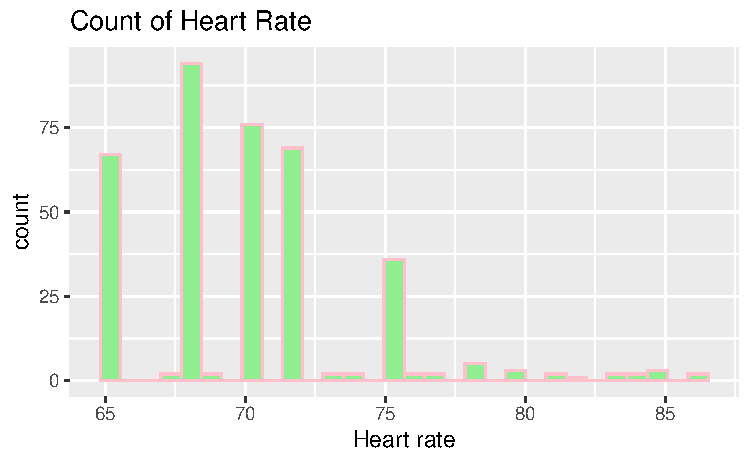
\includegraphics[width=0.7\linewidth]{SleepHelath_files/figure-latex/unnamed-chunk-7-1} \end{center}

\hypertarget{sleep-data-gender}{%
\section{Sleep Data Gender}\label{sleep-data-gender}}

\begin{Shaded}
\begin{Highlighting}[]
\NormalTok{sleep\_data }\SpecialCharTok{\%\textgreater{}\%}
  \FunctionTok{pivot\_longer}\NormalTok{(}\AttributeTok{cols =} \FunctionTok{c}\NormalTok{(Gender), }\AttributeTok{names\_to =} \StringTok{"variable"}\NormalTok{, }\AttributeTok{values\_to =} \StringTok{"value"}\NormalTok{) }\SpecialCharTok{\%\textgreater{}\%}
  \FunctionTok{group\_by}\NormalTok{(variable, value, sufficient\_sleep) }\SpecialCharTok{\%\textgreater{}\%}
  \FunctionTok{summarise}\NormalTok{(}\AttributeTok{count =} \FunctionTok{n}\NormalTok{()) }\SpecialCharTok{\%\textgreater{}\%}
  \FunctionTok{ggplot}\NormalTok{() }\SpecialCharTok{+}
  \FunctionTok{geom\_bar}\NormalTok{(}
    \AttributeTok{mapping =} \FunctionTok{aes}\NormalTok{(}\AttributeTok{x =}\NormalTok{ value, }\AttributeTok{y =}\NormalTok{ count, }\AttributeTok{fill =}\NormalTok{ sufficient\_sleep),}
    \AttributeTok{position =} \StringTok{"dodge"}\NormalTok{,  }
    \AttributeTok{alpha =} \FloatTok{0.6}\NormalTok{,}
    \AttributeTok{stat =} \StringTok{"identity"}
\NormalTok{  ) }\SpecialCharTok{+}
  \FunctionTok{facet\_wrap}\NormalTok{(}\SpecialCharTok{\textasciitilde{}}\NormalTok{ variable, }\AttributeTok{scales =} \StringTok{"free"}\NormalTok{) }\SpecialCharTok{+}
  \FunctionTok{labs}\NormalTok{(}\AttributeTok{title =} \StringTok{"Distribution of Sufficient Sleep by Gender"}\NormalTok{,}
       \AttributeTok{x =} \StringTok{"Value"}\NormalTok{, }
       \AttributeTok{y =} \StringTok{"Count"}\NormalTok{, }
       \AttributeTok{fill =} \StringTok{"Sufficient Sleep"}\NormalTok{)}
\end{Highlighting}
\end{Shaded}

\begin{center}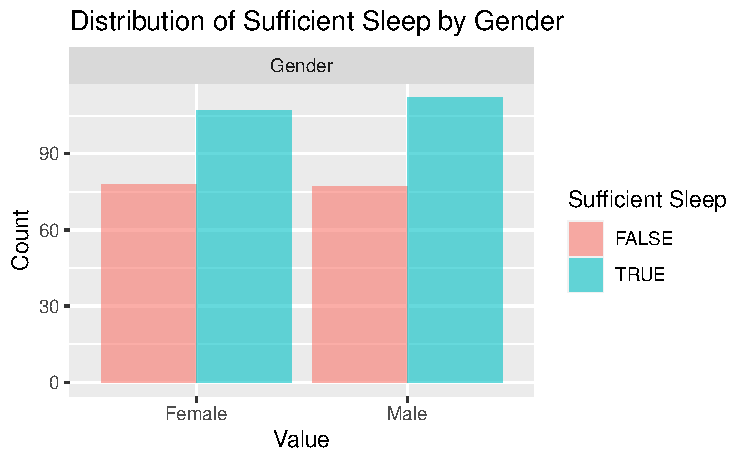
\includegraphics[width=0.7\linewidth]{SleepHelath_files/figure-latex/unnamed-chunk-8-1} \end{center}

\hypertarget{sleep-data-bmi}{%
\section{Sleep Data BMI}\label{sleep-data-bmi}}

\begin{Shaded}
\begin{Highlighting}[]
\NormalTok{sleep\_data }\SpecialCharTok{\%\textgreater{}\%}
  \FunctionTok{pivot\_longer}\NormalTok{(}\AttributeTok{cols =} \FunctionTok{c}\NormalTok{(BMI), }\AttributeTok{names\_to =} \StringTok{"variable"}\NormalTok{, }\AttributeTok{values\_to =} \StringTok{"value"}\NormalTok{) }\SpecialCharTok{\%\textgreater{}\%}
  \FunctionTok{mutate}\NormalTok{(}\AttributeTok{value =} \FunctionTok{ifelse}\NormalTok{(value }\SpecialCharTok{==} \StringTok{"Normal"}\NormalTok{, }\StringTok{"Normal Weight"}\NormalTok{, value)) }\SpecialCharTok{\%\textgreater{}\%}
  \FunctionTok{group\_by}\NormalTok{(variable, value, sufficient\_sleep) }\SpecialCharTok{\%\textgreater{}\%}
  \FunctionTok{summarise}\NormalTok{(}\AttributeTok{count =} \FunctionTok{n}\NormalTok{()) }\SpecialCharTok{\%\textgreater{}\%}
  \FunctionTok{ggplot}\NormalTok{() }\SpecialCharTok{+}
  \FunctionTok{geom\_bar}\NormalTok{(}
    \AttributeTok{mapping =} \FunctionTok{aes}\NormalTok{(}\AttributeTok{x =}\NormalTok{ value, }\AttributeTok{y =}\NormalTok{ count, }\AttributeTok{fill =}\NormalTok{ sufficient\_sleep),}
    \AttributeTok{position =} \StringTok{"dodge"}\NormalTok{,   }
    \AttributeTok{alpha =} \FloatTok{0.6}\NormalTok{,}
    \AttributeTok{stat =} \StringTok{"identity"}
\NormalTok{  ) }\SpecialCharTok{+}
  \FunctionTok{facet\_wrap}\NormalTok{(}\SpecialCharTok{\textasciitilde{}}\NormalTok{ variable, }\AttributeTok{scales =} \StringTok{"free"}\NormalTok{) }\SpecialCharTok{+}
  \FunctionTok{labs}\NormalTok{(}\AttributeTok{title =} \StringTok{"Distribution of Sufficient Sleep by BMI Category"}\NormalTok{,}
       \AttributeTok{x =} \StringTok{"Value"}\NormalTok{, }
       \AttributeTok{y =} \StringTok{"Count"}\NormalTok{, }
       \AttributeTok{fill =} \StringTok{"Sufficient Sleep"}\NormalTok{)}
\end{Highlighting}
\end{Shaded}

\begin{center}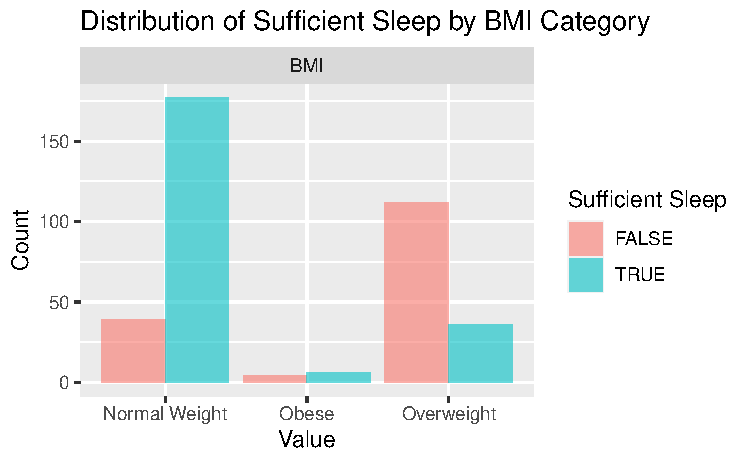
\includegraphics[width=0.7\linewidth]{SleepHelath_files/figure-latex/unnamed-chunk-9-1} \end{center}

\hypertarget{mode}{%
\section{Mode}\label{mode}}

\begin{Shaded}
\begin{Highlighting}[]
\NormalTok{mode\_gender }\OtherTok{\textless{}{-}} \FunctionTok{as.character}\NormalTok{(}\FunctionTok{names}\NormalTok{(}\FunctionTok{which.max}\NormalTok{(}\FunctionTok{table}\NormalTok{(sleep\_data}\SpecialCharTok{$}\NormalTok{Gender))))}
\NormalTok{mode\_occupation }\OtherTok{\textless{}{-}} \FunctionTok{as.character}\NormalTok{(}\FunctionTok{names}\NormalTok{(}\FunctionTok{which.max}\NormalTok{(}\FunctionTok{table}\NormalTok{(sleep\_data}\SpecialCharTok{$}\NormalTok{Occupation))))}
\NormalTok{mode\_bmi }\OtherTok{\textless{}{-}} \FunctionTok{as.character}\NormalTok{(}\FunctionTok{names}\NormalTok{(}\FunctionTok{which.max}\NormalTok{(}\FunctionTok{table}\NormalTok{(sleep\_data}\SpecialCharTok{$}\NormalTok{BMI))))}

\NormalTok{sleep\_data }\OtherTok{\textless{}{-}}\NormalTok{ sleep\_data }\SpecialCharTok{\%\textgreater{}\%}
\FunctionTok{mutate}\NormalTok{(}
  \AttributeTok{Gender =} \FunctionTok{if\_else}\NormalTok{(}\FunctionTok{is.na}\NormalTok{(Gender), mode\_gender, Gender),}
  \AttributeTok{Occupation =} \FunctionTok{if\_else}\NormalTok{(}\FunctionTok{is.na}\NormalTok{(Occupation), mode\_occupation, Occupation),}
  \AttributeTok{BMI =} \FunctionTok{if\_else}\NormalTok{(}\FunctionTok{is.na}\NormalTok{(BMI), mode\_bmi, BMI)}
\NormalTok{)}
\end{Highlighting}
\end{Shaded}

\hypertarget{sufficient-sleep}{%
\section{Sufficient Sleep}\label{sufficient-sleep}}

\begin{Shaded}
\begin{Highlighting}[]
\NormalTok{sleep\_data}\SpecialCharTok{$}\NormalTok{sufficient\_sleep }\OtherTok{\textless{}{-}} \FunctionTok{ifelse}\NormalTok{(sleep\_data}\SpecialCharTok{$}\NormalTok{Duration }\SpecialCharTok{\textgreater{}=} \DecValTok{7}\NormalTok{, }\StringTok{"Sufficient"}\NormalTok{, }\StringTok{"Insufficient"}\NormalTok{)}
\end{Highlighting}
\end{Shaded}

\hypertarget{saparate-train-test-set}{%
\section{Saparate Train, Test Set}\label{saparate-train-test-set}}

\begin{Shaded}
\begin{Highlighting}[]
\FunctionTok{set.seed}\NormalTok{(}\DecValTok{123}\NormalTok{)}
\NormalTok{train\_indices }\OtherTok{\textless{}{-}} \FunctionTok{createDataPartition}\NormalTok{(sleep\_data}\SpecialCharTok{$}\NormalTok{sufficient\_sleep, }\AttributeTok{p =} \FloatTok{0.7}\NormalTok{, }\AttributeTok{list =} \ConstantTok{FALSE}\NormalTok{)}
\NormalTok{trainingSet }\OtherTok{\textless{}{-}}\NormalTok{ sleep\_data[train\_indices, ]}
\NormalTok{testSet }\OtherTok{\textless{}{-}}\NormalTok{ sleep\_data[}\SpecialCharTok{{-}}\NormalTok{train\_indices, ]}

\NormalTok{trainingSet}\SpecialCharTok{$}\NormalTok{sufficient\_sleep }\OtherTok{\textless{}{-}} \FunctionTok{as.factor}\NormalTok{(trainingSet}\SpecialCharTok{$}\NormalTok{sufficient\_sleep)}
\NormalTok{testSet}\SpecialCharTok{$}\NormalTok{sufficient\_sleep }\OtherTok{\textless{}{-}} \FunctionTok{as.factor}\NormalTok{(testSet}\SpecialCharTok{$}\NormalTok{sufficient\_sleep)}

\NormalTok{training\_Outcomes }\OtherTok{\textless{}{-}}\NormalTok{ trainingSet}\SpecialCharTok{$}\NormalTok{sufficient\_sleep}
\NormalTok{test\_Outcomes }\OtherTok{\textless{}{-}}\NormalTok{ testSet}\SpecialCharTok{$}\NormalTok{sufficient\_sleep}
\end{Highlighting}
\end{Shaded}

\hypertarget{train}{%
\section{Train}\label{train}}

\begin{Shaded}
\begin{Highlighting}[]
\NormalTok{model }\OtherTok{\textless{}{-}} \FunctionTok{glm}\NormalTok{(sufficient\_sleep }\SpecialCharTok{\textasciitilde{}}\NormalTok{ Age }\SpecialCharTok{+}\NormalTok{ Gender }\SpecialCharTok{+}\NormalTok{ Occupation }\SpecialCharTok{+}\NormalTok{ Physical }\SpecialCharTok{+}\NormalTok{ DSteps }\SpecialCharTok{+}\NormalTok{ BMI, }\AttributeTok{data =}\NormalTok{ trainingSet, }\AttributeTok{family =}\NormalTok{ binomial)}
\end{Highlighting}
\end{Shaded}

\hypertarget{predict}{%
\section{Predict}\label{predict}}

\begin{Shaded}
\begin{Highlighting}[]
\NormalTok{predictions }\OtherTok{\textless{}{-}} \FunctionTok{predict}\NormalTok{(model, }\AttributeTok{newdata =}\NormalTok{ testSet, }\AttributeTok{type =} \StringTok{"response"}\NormalTok{)}
\end{Highlighting}
\end{Shaded}

\hypertarget{test}{%
\section{Test}\label{test}}

\begin{Shaded}
\begin{Highlighting}[]
\NormalTok{threshold }\OtherTok{\textless{}{-}} \FloatTok{0.5}  
\NormalTok{predicted\_classes }\OtherTok{\textless{}{-}} \FunctionTok{as.factor}\NormalTok{(}\FunctionTok{ifelse}\NormalTok{(predictions }\SpecialCharTok{\textgreater{}=}\NormalTok{ threshold, }\StringTok{"Sufficient"}\NormalTok{, }\StringTok{"Insufficient"}\NormalTok{))}
\NormalTok{actual\_classes }\OtherTok{\textless{}{-}}\NormalTok{ test\_Outcomes}
\NormalTok{accuracy }\OtherTok{\textless{}{-}} \FunctionTok{sum}\NormalTok{(predicted\_classes }\SpecialCharTok{==}\NormalTok{ actual\_classes) }\SpecialCharTok{/} \FunctionTok{length}\NormalTok{(actual\_classes)}
\FunctionTok{print}\NormalTok{(}\FunctionTok{paste}\NormalTok{(}\StringTok{"Accuracy:"}\NormalTok{, accuracy))}
\end{Highlighting}
\end{Shaded}

\begin{verbatim}
## [1] "Accuracy: 0.981981981981982"
\end{verbatim}

\begin{Shaded}
\begin{Highlighting}[]
\NormalTok{model\_1\_preds }\OtherTok{\textless{}{-}}\NormalTok{ testSet }\SpecialCharTok{\%\textgreater{}\%}
  \FunctionTok{add\_predictions}\NormalTok{(model, }\AttributeTok{type =} \StringTok{"response"}\NormalTok{) }\SpecialCharTok{\%\textgreater{}\%}
  \FunctionTok{mutate}\NormalTok{(}
    \AttributeTok{outcome =} \FunctionTok{as.factor}\NormalTok{(}\FunctionTok{if\_else}\NormalTok{(}\AttributeTok{condition =}\NormalTok{ pred }\SpecialCharTok{\textgreater{}}\NormalTok{ threshold, }
                      \StringTok{"Sufficient"}\NormalTok{, }\StringTok{"Insufficient"}\NormalTok{))}
\NormalTok{  )}
\end{Highlighting}
\end{Shaded}

\#Hypothesis

\begin{Shaded}
\begin{Highlighting}[]
\NormalTok{Sleep\_health\_and\_lifestyle\_dataset\_renamed }\OtherTok{\textless{}{-}}\NormalTok{ Sleep\_health\_and\_lifestyle\_dataset }\SpecialCharTok{\%\textgreater{}\%}
  \FunctionTok{rename}\NormalTok{( }\AttributeTok{Duration =} \StringTok{\textquotesingle{}Sleep Duration\textquotesingle{}}\NormalTok{,}
          \AttributeTok{Stress =} \StringTok{\textquotesingle{}Stress Level\textquotesingle{}}\NormalTok{,}
          \AttributeTok{Physical =} \StringTok{\textquotesingle{}Physical Activity Level\textquotesingle{}}\NormalTok{ ,}
          \AttributeTok{Quality =} \StringTok{\textquotesingle{}Quality of Sleep\textquotesingle{}}\NormalTok{ ,}
          \AttributeTok{BMI=} \StringTok{\textquotesingle{}BMI Category\textquotesingle{}}\NormalTok{ ,}
          \AttributeTok{BPressure =} \StringTok{\textquotesingle{}Blood Pressure\textquotesingle{}}\NormalTok{ ,}
          \AttributeTok{HRate =} \StringTok{\textquotesingle{}Heart Rate\textquotesingle{}}\NormalTok{ ,}
          \AttributeTok{DSteps =} \StringTok{\textquotesingle{}Daily Steps\textquotesingle{}}\NormalTok{ ,}
          \AttributeTok{Disorder =} \StringTok{\textquotesingle{}Sleep Disorder\textquotesingle{}}\NormalTok{ )}
\end{Highlighting}
\end{Shaded}

\begin{Shaded}
\begin{Highlighting}[]
\NormalTok{Sleep\_health\_and\_lifestyle\_dataset\_renamed}\SpecialCharTok{$}\NormalTok{BMI[Sleep\_health\_and\_lifestyle\_dataset\_renamed}\SpecialCharTok{$}\NormalTok{BMI }\SpecialCharTok{==} \StringTok{"Overweight"}\NormalTok{] }\OtherTok{\textless{}{-}} \StringTok{"High"}
\NormalTok{Sleep\_health\_and\_lifestyle\_dataset\_renamed}\SpecialCharTok{$}\NormalTok{BMI[Sleep\_health\_and\_lifestyle\_dataset\_renamed}\SpecialCharTok{$}\NormalTok{BMI }\SpecialCharTok{==} \StringTok{"Obese"}\NormalTok{] }\OtherTok{\textless{}{-}} \StringTok{"High"}
\NormalTok{Sleep\_health\_and\_lifestyle\_dataset\_renamed}\SpecialCharTok{$}\NormalTok{BMI[Sleep\_health\_and\_lifestyle\_dataset\_renamed}\SpecialCharTok{$}\NormalTok{BMI }\SpecialCharTok{==} \StringTok{"Normal Weight"}\NormalTok{] }\OtherTok{\textless{}{-}} \StringTok{"Normal"}
\end{Highlighting}
\end{Shaded}

\begin{Shaded}
\begin{Highlighting}[]
\NormalTok{Sleep\_health\_and\_lifestyle\_dataset\_renamed }\SpecialCharTok{\%\textgreater{}\%}
  \FunctionTok{filter}\NormalTok{(BMI }\SpecialCharTok{==} \StringTok{"Normal"} \SpecialCharTok{|}\NormalTok{ BMI }\SpecialCharTok{==} \StringTok{"High"}\NormalTok{) }\SpecialCharTok{\%\textgreater{}\%}
  \FunctionTok{ggplot}\NormalTok{() }\SpecialCharTok{+}
  \FunctionTok{geom\_histogram}\NormalTok{( }
    \AttributeTok{mapping =} \FunctionTok{aes}\NormalTok{(}\AttributeTok{x =}\NormalTok{ Duration, }\AttributeTok{fill =}\NormalTok{ BMI), }
    \AttributeTok{position =} \StringTok{"identity"}\NormalTok{,}
\AttributeTok{alpha =} \FloatTok{0.5}
\NormalTok{  )}
\end{Highlighting}
\end{Shaded}

\begin{verbatim}
## `stat_bin()` using `bins = 30`. Pick better value with `binwidth`.
\end{verbatim}

\begin{center}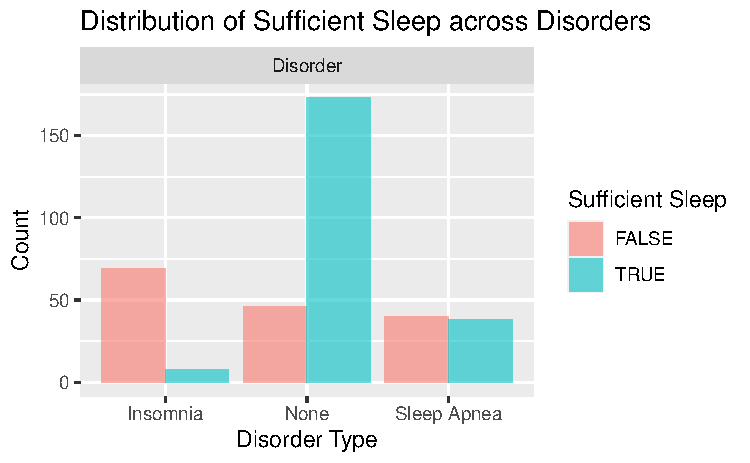
\includegraphics[width=0.7\linewidth]{SleepHelath_files/figure-latex/unnamed-chunk-18-1} \end{center}

\begin{Shaded}
\begin{Highlighting}[]
\NormalTok{Sleep\_health\_and\_lifestyle\_dataset\_renamed }\SpecialCharTok{\%\textgreater{}\%}
  \FunctionTok{filter}\NormalTok{(BMI }\SpecialCharTok{==} \StringTok{"Normal"} \SpecialCharTok{|}\NormalTok{ BMI }\SpecialCharTok{==} \StringTok{"High"}\NormalTok{) }\SpecialCharTok{\%\textgreater{}\%}
  \FunctionTok{ggplot}\NormalTok{() }\SpecialCharTok{+}
  \FunctionTok{geom\_histogram}\NormalTok{( }
    \AttributeTok{mapping =} \FunctionTok{aes}\NormalTok{(}\AttributeTok{x =}\NormalTok{ Duration, }\AttributeTok{y=}\NormalTok{ ..density.., }\AttributeTok{fill =}\NormalTok{ BMI), }
    \AttributeTok{position =} \StringTok{"identity"}\NormalTok{,}
\AttributeTok{alpha =} \FloatTok{0.5}
\NormalTok{  )}
\end{Highlighting}
\end{Shaded}

\begin{verbatim}
## Warning: The dot-dot notation (`..density..`) was deprecated in ggplot2 3.4.0.
## i Please use `after_stat(density)` instead.
## This warning is displayed once every 8 hours.
## Call `lifecycle::last_lifecycle_warnings()` to see where this warning was
## generated.
\end{verbatim}

\begin{verbatim}
## `stat_bin()` using `bins = 30`. Pick better value with `binwidth`.
\end{verbatim}

\begin{center}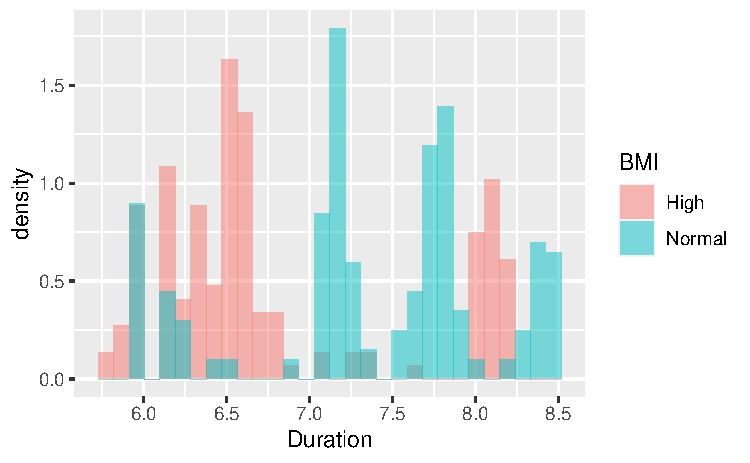
\includegraphics[width=0.7\linewidth]{SleepHelath_files/figure-latex/unnamed-chunk-19-1} \end{center}

\begin{Shaded}
\begin{Highlighting}[]
\NormalTok{Sleep\_health\_and\_lifestyle\_dataset\_renamed }\SpecialCharTok{\%\textgreater{}\%}
  \FunctionTok{filter}\NormalTok{(BMI }\SpecialCharTok{==} \StringTok{"Normal"} \SpecialCharTok{|}\NormalTok{ BMI }\SpecialCharTok{==} \StringTok{"High"}\NormalTok{) }\SpecialCharTok{\%\textgreater{}\%}
  \FunctionTok{ggplot}\NormalTok{() }\SpecialCharTok{+}
  \FunctionTok{geom\_density}\NormalTok{( }
    \AttributeTok{mapping =} \FunctionTok{aes}\NormalTok{(}\AttributeTok{x =}\NormalTok{ Duration, }\AttributeTok{fill =}\NormalTok{ BMI), }
    \AttributeTok{position =} \StringTok{"identity"}\NormalTok{,}
\AttributeTok{alpha =} \FloatTok{0.5}
\NormalTok{  )}
\end{Highlighting}
\end{Shaded}

\begin{center}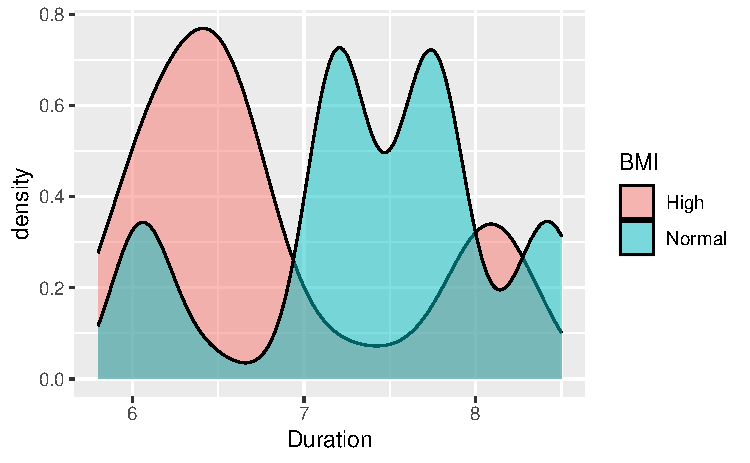
\includegraphics[width=0.7\linewidth]{SleepHelath_files/figure-latex/unnamed-chunk-20-1} \end{center}

\begin{Shaded}
\begin{Highlighting}[]
\NormalTok{Sleep\_health\_and\_lifestyle\_dataset\_renamed }\SpecialCharTok{\%\textgreater{}\%}
\FunctionTok{summarize}\NormalTok{(}
\AttributeTok{mean =} \FunctionTok{mean}\NormalTok{(Duration),}
\AttributeTok{median =} \FunctionTok{median}\NormalTok{(Duration), }
\AttributeTok{standard\_deviation =} \FunctionTok{sd}\NormalTok{(Duration), }
\AttributeTok{minimum =} \FunctionTok{min}\NormalTok{(Duration),}
\AttributeTok{maximum =} \FunctionTok{max}\NormalTok{(Duration)}
\NormalTok{)}
\end{Highlighting}
\end{Shaded}

\begin{longtable}[]{@{}rrrrr@{}}
\toprule\noalign{}
mean & median & standard\_deviation & minimum & maximum \\
\midrule\noalign{}
\endhead
\bottomrule\noalign{}
\endlastfoot
7.132086 & 7.2 & 0.7956567 & 5.8 & 8.5 \\
\end{longtable}

\begin{Shaded}
\begin{Highlighting}[]
\NormalTok{Model }\OtherTok{\textless{}{-}} \FunctionTok{lm}\NormalTok{(Duration }\SpecialCharTok{\textasciitilde{}}\NormalTok{ BMI, }\AttributeTok{data =}\NormalTok{ Sleep\_health\_and\_lifestyle\_dataset\_renamed)}
\NormalTok{Simulation\_results }\OtherTok{\textless{}{-}}
\NormalTok{  Sleep\_health\_and\_lifestyle\_dataset\_renamed }\SpecialCharTok{\%\textgreater{}\%}
  \FunctionTok{specify}\NormalTok{(Duration }\SpecialCharTok{\textasciitilde{}}\NormalTok{ BMI) }\SpecialCharTok{\%\textgreater{}\%}
  \FunctionTok{hypothesize}\NormalTok{(}\AttributeTok{null =} \StringTok{"independence"}\NormalTok{) }\SpecialCharTok{\%\textgreater{}\%}
  \FunctionTok{generate}\NormalTok{(}\AttributeTok{reps =} \DecValTok{1000}\NormalTok{, }\AttributeTok{type =} \StringTok{"permute"}\NormalTok{) }\SpecialCharTok{\%\textgreater{}\%} 
  \FunctionTok{calculate}\NormalTok{(}\AttributeTok{stat =} \StringTok{"diff in means"}\NormalTok{, }\AttributeTok{order =} \FunctionTok{c}\NormalTok{(}\StringTok{"Normal"}\NormalTok{, }\StringTok{"High"}\NormalTok{))}
\end{Highlighting}
\end{Shaded}

\begin{Shaded}
\begin{Highlighting}[]
\NormalTok{Shl\_obs\_stat }\OtherTok{\textless{}{-}}
\NormalTok{  Sleep\_health\_and\_lifestyle\_dataset\_renamed }\SpecialCharTok{\%\textgreater{}\%}
  \FunctionTok{specify}\NormalTok{(}\AttributeTok{formula =}\NormalTok{ Duration }\SpecialCharTok{\textasciitilde{}}\NormalTok{ BMI) }\SpecialCharTok{\%\textgreater{}\%}
  \FunctionTok{calculate}\NormalTok{(}\AttributeTok{stat =} \StringTok{"diff in means"}\NormalTok{, }\AttributeTok{order =} \FunctionTok{c}\NormalTok{(}\StringTok{"Normal"}\NormalTok{,}\StringTok{"High"}\NormalTok{))}
\end{Highlighting}
\end{Shaded}

\begin{Shaded}
\begin{Highlighting}[]
\NormalTok{Shl\_null }\OtherTok{\textless{}{-}}\NormalTok{ Sleep\_health\_and\_lifestyle\_dataset\_renamed }\SpecialCharTok{\%\textgreater{}\%}
  \FunctionTok{specify}\NormalTok{(Duration }\SpecialCharTok{\textasciitilde{}}\NormalTok{ BMI) }\SpecialCharTok{\%\textgreater{}\%}
  \FunctionTok{hypothesize}\NormalTok{(}\AttributeTok{null =} \StringTok{"independence"}\NormalTok{) }\SpecialCharTok{\%\textgreater{}\%}
  \FunctionTok{generate}\NormalTok{(}\AttributeTok{reps =} \DecValTok{1000}\NormalTok{, }\AttributeTok{type =} \StringTok{"permute"}\NormalTok{)}
\end{Highlighting}
\end{Shaded}

\begin{Shaded}
\begin{Highlighting}[]
\NormalTok{Shl\_null }\SpecialCharTok{\%\textgreater{}\%}
  \FunctionTok{get\_p\_value}\NormalTok{(}\AttributeTok{obs\_stat =}\NormalTok{ Shl\_obs\_stat, }\AttributeTok{direction =} \StringTok{"right"}\NormalTok{)}
\end{Highlighting}
\end{Shaded}

\begin{longtable}[]{@{}r@{}}
\toprule\noalign{}
p\_value \\
\midrule\noalign{}
\endhead
\bottomrule\noalign{}
\endlastfoot
1 \\
\end{longtable}

\begin{Shaded}
\begin{Highlighting}[]
\NormalTok{Shl\_null }\SpecialCharTok{\%\textgreater{}\%} \FunctionTok{get\_p\_value}\NormalTok{(}\AttributeTok{obs\_stat =}\NormalTok{ Shl\_obs\_stat, }\AttributeTok{direction =} \StringTok{"right"}\NormalTok{)}
\end{Highlighting}
\end{Shaded}

\begin{longtable}[]{@{}r@{}}
\toprule\noalign{}
p\_value \\
\midrule\noalign{}
\endhead
\bottomrule\noalign{}
\endlastfoot
1 \\
\end{longtable}

\begin{Shaded}
\begin{Highlighting}[]
\NormalTok{p\_value }\OtherTok{\textless{}{-}}\NormalTok{ Shl\_null }\SpecialCharTok{\%\textgreater{}\%} \FunctionTok{get\_p\_value}\NormalTok{(}\AttributeTok{obs\_stat =}\NormalTok{ Shl\_obs\_stat, }\AttributeTok{direction =} \StringTok{"right"}\NormalTok{)}
\end{Highlighting}
\end{Shaded}

\begin{Shaded}
\begin{Highlighting}[]
\NormalTok{Sleep\_health\_and\_lifestyle\_dataset\_renamed }\SpecialCharTok{\%\textgreater{}\%}
  \FunctionTok{filter}\NormalTok{(BMI }\SpecialCharTok{==} \StringTok{"Normal"} \SpecialCharTok{|}\NormalTok{ BMI }\SpecialCharTok{==} \StringTok{"High"}\NormalTok{) }\SpecialCharTok{\%\textgreater{}\%}
  \FunctionTok{ggplot}\NormalTok{() }\SpecialCharTok{+}
  \FunctionTok{geom\_density}\NormalTok{(}\AttributeTok{mapping =} \FunctionTok{aes}\NormalTok{(}\AttributeTok{x =}\NormalTok{ Duration, }\AttributeTok{fill =}\NormalTok{ BMI), }\AttributeTok{position =} \StringTok{"identity"}\NormalTok{, }\AttributeTok{alpha =} \FloatTok{0.5}\NormalTok{) }\SpecialCharTok{+}
  \FunctionTok{geom\_text}\NormalTok{(}\FunctionTok{aes}\NormalTok{(}\AttributeTok{x =} \ConstantTok{Inf}\NormalTok{, }\AttributeTok{y =} \ConstantTok{Inf}\NormalTok{, }\AttributeTok{label =} \FunctionTok{paste}\NormalTok{(}\StringTok{"p{-}value ="}\NormalTok{, }\FunctionTok{round}\NormalTok{(p\_value, }\DecValTok{3}\NormalTok{))),}
            \AttributeTok{hjust =} \DecValTok{1}\NormalTok{, }\AttributeTok{vjust =} \DecValTok{1}\NormalTok{, }\AttributeTok{color =} \StringTok{"red"}\NormalTok{) }\SpecialCharTok{+}
  \FunctionTok{labs}\NormalTok{(}\AttributeTok{title =} \StringTok{"Duration vs. BMI Density Plot"}\NormalTok{,}
       \AttributeTok{x =} \StringTok{"Duration"}\NormalTok{,}
       \AttributeTok{y =} \StringTok{"Density"}\NormalTok{) }\SpecialCharTok{+}
  \FunctionTok{theme\_minimal}\NormalTok{()}
\end{Highlighting}
\end{Shaded}

\begin{center}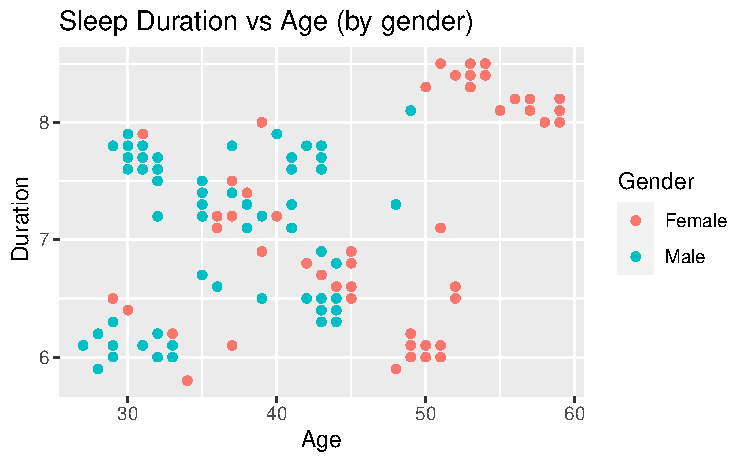
\includegraphics[width=0.7\linewidth]{SleepHelath_files/figure-latex/unnamed-chunk-27-1} \end{center}

\hypertarget{part-2-data-visualization}{%
\subsubsection{Part 2 Data
Visualization}\label{part-2-data-visualization}}

\begin{Shaded}
\begin{Highlighting}[]
\NormalTok{Sleep\_health\_and\_lifestyle\_dataset\_renamed }\OtherTok{\textless{}{-}}\NormalTok{ Sleep\_health\_and\_lifestyle\_dataset}\SpecialCharTok{\%\textgreater{}\%}
  \FunctionTok{rename}\NormalTok{( }\AttributeTok{ID =} \StringTok{"Person ID"}\NormalTok{,}
          \AttributeTok{Duration =} \StringTok{\textquotesingle{}Sleep Duration\textquotesingle{}}\NormalTok{,}
          \AttributeTok{Stress =} \StringTok{\textquotesingle{}Stress Level\textquotesingle{}}\NormalTok{,}
          \AttributeTok{Physical =} \StringTok{\textquotesingle{}Physical Activity Level\textquotesingle{}}\NormalTok{ ,}
          \AttributeTok{Quality =} \StringTok{\textquotesingle{}Quality of Sleep\textquotesingle{}}\NormalTok{ ,}
          \AttributeTok{BMI=} \StringTok{\textquotesingle{}BMI Category\textquotesingle{}}\NormalTok{ ,}
          \AttributeTok{BPressure =} \StringTok{\textquotesingle{}Blood Pressure\textquotesingle{}}\NormalTok{ ,}
          \AttributeTok{HRate =} \StringTok{\textquotesingle{}Heart Rate\textquotesingle{}}\NormalTok{ ,}
          \AttributeTok{DSteps =} \StringTok{\textquotesingle{}Daily Steps\textquotesingle{}}\NormalTok{ ,}
          \AttributeTok{Disorder =} \StringTok{\textquotesingle{}Sleep Disorder\textquotesingle{}}\NormalTok{ )}
\end{Highlighting}
\end{Shaded}

\begin{Shaded}
\begin{Highlighting}[]
\NormalTok{Sleep\_health\_and\_lifestyle\_dataset\_renamed }\SpecialCharTok{\%\textgreater{}\%}
  \FunctionTok{ggplot}\NormalTok{()}\SpecialCharTok{+}
  \FunctionTok{geom\_point}\NormalTok{( }\AttributeTok{mapping =} \FunctionTok{aes}\NormalTok{( }\AttributeTok{x =}\NormalTok{ Age , }\AttributeTok{y =}\NormalTok{ Duration, }\AttributeTok{color =}\NormalTok{ Gender))}\SpecialCharTok{+}
  \FunctionTok{labs}\NormalTok{(}
   \AttributeTok{title =} \StringTok{"Sleep Duration vs Age (by gender)"}\NormalTok{,}
   \AttributeTok{x=} \StringTok{"Age"}\NormalTok{, }\AttributeTok{y =} \StringTok{" Duration"}\NormalTok{)}
\end{Highlighting}
\end{Shaded}

\begin{center}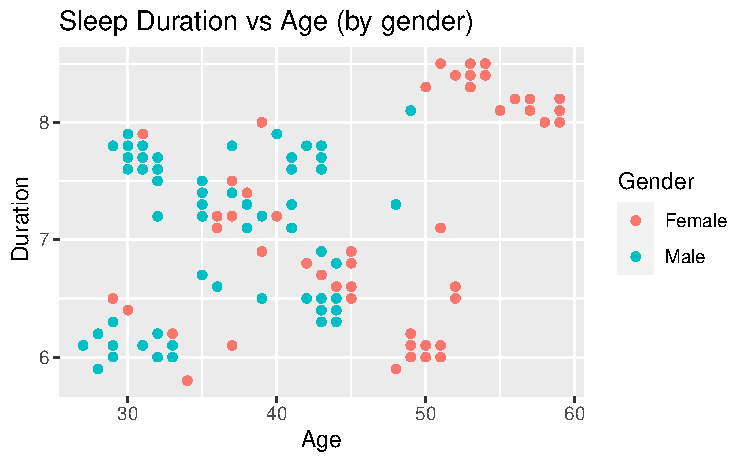
\includegraphics[width=0.7\linewidth]{SleepHelath_files/figure-latex/unnamed-chunk-29-1} \end{center}

\begin{Shaded}
\begin{Highlighting}[]
\NormalTok{model\_2 }\OtherTok{\textless{}{-}} \FunctionTok{lm}\NormalTok{(Duration }\SpecialCharTok{\textasciitilde{}}\NormalTok{ Physical,Sleep\_health\_and\_lifestyle\_dataset\_renamed)}
\end{Highlighting}
\end{Shaded}

\begin{Shaded}
\begin{Highlighting}[]
\NormalTok{model\_2}\SpecialCharTok{$}\NormalTok{coefficients}
\end{Highlighting}
\end{Shaded}

\begin{verbatim}
## (Intercept)    Physical 
## 6.652127945 0.008111349
\end{verbatim}

\begin{Shaded}
\begin{Highlighting}[]
\NormalTok{Sleep\_health\_and\_lifestyle\_dataset\_renamed }\SpecialCharTok{\%\textgreater{}\%}
  \FunctionTok{ggplot}\NormalTok{() }\SpecialCharTok{+}
  \FunctionTok{geom\_point}\NormalTok{(}\AttributeTok{mapping =} \FunctionTok{aes}\NormalTok{(}\AttributeTok{x =}\NormalTok{ Physical, }\AttributeTok{y =}\NormalTok{ Duration), }\AttributeTok{bin =} \DecValTok{10}\NormalTok{) }\SpecialCharTok{+}
  \FunctionTok{geom\_abline}\NormalTok{(}\AttributeTok{slope =}\NormalTok{ model\_2}\SpecialCharTok{$}\NormalTok{coefficients[}\DecValTok{2}\NormalTok{], }
              \AttributeTok{intercept =}\NormalTok{ model\_2}\SpecialCharTok{$}\NormalTok{coefficients[}\DecValTok{1}\NormalTok{])}\SpecialCharTok{+}
   \FunctionTok{labs}\NormalTok{(}\AttributeTok{x =} \StringTok{"Physical Activity Level"}\NormalTok{, }\AttributeTok{y =} \StringTok{"Sleep Duration"}\NormalTok{,}
                    \AttributeTok{title =} \StringTok{"physical activity level vs sleep duration"}\NormalTok{ )}
\end{Highlighting}
\end{Shaded}

\begin{center}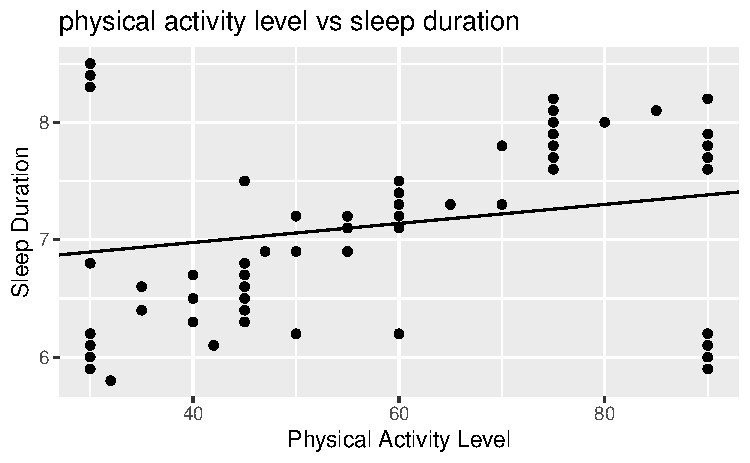
\includegraphics[width=0.7\linewidth]{SleepHelath_files/figure-latex/unnamed-chunk-32-1} \end{center}

\hypertarget{data-wrangling}{%
\subsubsection{Data Wrangling}\label{data-wrangling}}

\begin{Shaded}
\begin{Highlighting}[]
\NormalTok{Sleep\_health\_and\_lifestyle\_dataset\_renamed}\SpecialCharTok{$}\NormalTok{BMI[Sleep\_health\_and\_lifestyle\_dataset\_renamed}\SpecialCharTok{$}\NormalTok{BMI }\SpecialCharTok{==} \StringTok{"Overweight"}\NormalTok{] }\OtherTok{\textless{}{-}} \StringTok{"Fat"}
\NormalTok{Sleep\_health\_and\_lifestyle\_dataset\_renamed}\SpecialCharTok{$}\NormalTok{BMI[Sleep\_health\_and\_lifestyle\_dataset\_renamed}\SpecialCharTok{$}\NormalTok{BMI }\SpecialCharTok{==} \StringTok{"Obese"}\NormalTok{] }\OtherTok{\textless{}{-}} \StringTok{"Fat"}
\NormalTok{Sleep\_health\_and\_lifestyle\_dataset\_renamed}\SpecialCharTok{$}\NormalTok{BMI[Sleep\_health\_and\_lifestyle\_dataset\_renamed}\SpecialCharTok{$}\NormalTok{BMI }\SpecialCharTok{==} \StringTok{"Normal Weight"}\NormalTok{] }\OtherTok{\textless{}{-}} \StringTok{"Normal"}
\end{Highlighting}
\end{Shaded}

\begin{Shaded}
\begin{Highlighting}[]
\FunctionTok{head}\NormalTok{(Sleep\_health\_and\_lifestyle\_dataset\_renamed) }\SpecialCharTok{\%\textgreater{}\%}
  \FunctionTok{select}\NormalTok{(ID, HRate, Duration, Gender, Age, Occupation, Physical, BMI, Quality) }\SpecialCharTok{\%\textgreater{}\%}
  \FunctionTok{arrange}\NormalTok{(Duration)}
\end{Highlighting}
\end{Shaded}

\begin{longtable}[]{@{}
  >{\raggedright\arraybackslash}p{(\columnwidth - 16\tabcolsep) * \real{0.0405}}
  >{\raggedleft\arraybackslash}p{(\columnwidth - 16\tabcolsep) * \real{0.0811}}
  >{\raggedleft\arraybackslash}p{(\columnwidth - 16\tabcolsep) * \real{0.1216}}
  >{\raggedright\arraybackslash}p{(\columnwidth - 16\tabcolsep) * \real{0.0946}}
  >{\raggedleft\arraybackslash}p{(\columnwidth - 16\tabcolsep) * \real{0.0541}}
  >{\raggedright\arraybackslash}p{(\columnwidth - 16\tabcolsep) * \real{0.2838}}
  >{\raggedleft\arraybackslash}p{(\columnwidth - 16\tabcolsep) * \real{0.1216}}
  >{\raggedright\arraybackslash}p{(\columnwidth - 16\tabcolsep) * \real{0.0946}}
  >{\raggedleft\arraybackslash}p{(\columnwidth - 16\tabcolsep) * \real{0.1081}}@{}}
\toprule\noalign{}
\begin{minipage}[b]{\linewidth}\raggedright
ID
\end{minipage} & \begin{minipage}[b]{\linewidth}\raggedleft
HRate
\end{minipage} & \begin{minipage}[b]{\linewidth}\raggedleft
Duration
\end{minipage} & \begin{minipage}[b]{\linewidth}\raggedright
Gender
\end{minipage} & \begin{minipage}[b]{\linewidth}\raggedleft
Age
\end{minipage} & \begin{minipage}[b]{\linewidth}\raggedright
Occupation
\end{minipage} & \begin{minipage}[b]{\linewidth}\raggedleft
Physical
\end{minipage} & \begin{minipage}[b]{\linewidth}\raggedright
BMI
\end{minipage} & \begin{minipage}[b]{\linewidth}\raggedleft
Quality
\end{minipage} \\
\midrule\noalign{}
\endhead
\bottomrule\noalign{}
\endlastfoot
4 & 85 & 5.9 & Male & 28 & Sales Representative & 30 & Fat & 4 \\
5 & 85 & 5.9 & Male & 28 & Sales Representative & 30 & Fat & 4 \\
6 & 85 & 5.9 & Male & 28 & Software Engineer & 30 & Fat & 4 \\
1 & 77 & 6.1 & Male & 27 & Software Engineer & 42 & Fat & 6 \\
2 & 75 & 6.2 & Male & 28 & Doctor & 60 & Normal & 6 \\
3 & 75 & 6.2 & Male & 28 & Doctor & 60 & Normal & 6 \\
\end{longtable}

\begin{Shaded}
\begin{Highlighting}[]
\FunctionTok{tail}\NormalTok{(Sleep\_health\_and\_lifestyle\_dataset\_renamed) }\SpecialCharTok{\%\textgreater{}\%}
 \FunctionTok{select}\NormalTok{(ID, HRate, Duration, Gender, Age, Occupation, Physical, BMI, Quality) }\SpecialCharTok{\%\textgreater{}\%}
  \FunctionTok{arrange}\NormalTok{(Duration) }\SpecialCharTok{\%\textgreater{}\%}
  \FunctionTok{filter}\NormalTok{(Gender }\SpecialCharTok{==} \StringTok{\textquotesingle{}Female\textquotesingle{}}\NormalTok{)}
\end{Highlighting}
\end{Shaded}

\begin{longtable}[]{@{}lrrlrlrlr@{}}
\toprule\noalign{}
ID & HRate & Duration & Gender & Age & Occupation & Physical & BMI &
Quality \\
\midrule\noalign{}
\endhead
\bottomrule\noalign{}
\endlastfoot
371 & 68 & 8.0 & Female & 59 & Nurse & 75 & Fat & 9 \\
369 & 68 & 8.1 & Female & 59 & Nurse & 75 & Fat & 9 \\
370 & 68 & 8.1 & Female & 59 & Nurse & 75 & Fat & 9 \\
372 & 68 & 8.1 & Female & 59 & Nurse & 75 & Fat & 9 \\
373 & 68 & 8.1 & Female & 59 & Nurse & 75 & Fat & 9 \\
374 & 68 & 8.1 & Female & 59 & Nurse & 75 & Fat & 9 \\
\end{longtable}

\begin{Shaded}
\begin{Highlighting}[]
\FunctionTok{head}\NormalTok{(Sleep\_health\_and\_lifestyle\_dataset\_renamed) }\SpecialCharTok{\%\textgreater{}\%}
 \FunctionTok{select}\NormalTok{(ID, HRate, Duration, Gender, Age, Occupation, Physical, BMI, Quality) }\SpecialCharTok{\%\textgreater{}\%}
  \FunctionTok{arrange}\NormalTok{(Duration) }\SpecialCharTok{\%\textgreater{}\%}
  \FunctionTok{filter}\NormalTok{(Gender }\SpecialCharTok{==} \StringTok{\textquotesingle{}Male\textquotesingle{}}\NormalTok{)}
\end{Highlighting}
\end{Shaded}

\begin{longtable}[]{@{}
  >{\raggedright\arraybackslash}p{(\columnwidth - 16\tabcolsep) * \real{0.0405}}
  >{\raggedleft\arraybackslash}p{(\columnwidth - 16\tabcolsep) * \real{0.0811}}
  >{\raggedleft\arraybackslash}p{(\columnwidth - 16\tabcolsep) * \real{0.1216}}
  >{\raggedright\arraybackslash}p{(\columnwidth - 16\tabcolsep) * \real{0.0946}}
  >{\raggedleft\arraybackslash}p{(\columnwidth - 16\tabcolsep) * \real{0.0541}}
  >{\raggedright\arraybackslash}p{(\columnwidth - 16\tabcolsep) * \real{0.2838}}
  >{\raggedleft\arraybackslash}p{(\columnwidth - 16\tabcolsep) * \real{0.1216}}
  >{\raggedright\arraybackslash}p{(\columnwidth - 16\tabcolsep) * \real{0.0946}}
  >{\raggedleft\arraybackslash}p{(\columnwidth - 16\tabcolsep) * \real{0.1081}}@{}}
\toprule\noalign{}
\begin{minipage}[b]{\linewidth}\raggedright
ID
\end{minipage} & \begin{minipage}[b]{\linewidth}\raggedleft
HRate
\end{minipage} & \begin{minipage}[b]{\linewidth}\raggedleft
Duration
\end{minipage} & \begin{minipage}[b]{\linewidth}\raggedright
Gender
\end{minipage} & \begin{minipage}[b]{\linewidth}\raggedleft
Age
\end{minipage} & \begin{minipage}[b]{\linewidth}\raggedright
Occupation
\end{minipage} & \begin{minipage}[b]{\linewidth}\raggedleft
Physical
\end{minipage} & \begin{minipage}[b]{\linewidth}\raggedright
BMI
\end{minipage} & \begin{minipage}[b]{\linewidth}\raggedleft
Quality
\end{minipage} \\
\midrule\noalign{}
\endhead
\bottomrule\noalign{}
\endlastfoot
4 & 85 & 5.9 & Male & 28 & Sales Representative & 30 & Fat & 4 \\
5 & 85 & 5.9 & Male & 28 & Sales Representative & 30 & Fat & 4 \\
6 & 85 & 5.9 & Male & 28 & Software Engineer & 30 & Fat & 4 \\
1 & 77 & 6.1 & Male & 27 & Software Engineer & 42 & Fat & 6 \\
2 & 75 & 6.2 & Male & 28 & Doctor & 60 & Normal & 6 \\
3 & 75 & 6.2 & Male & 28 & Doctor & 60 & Normal & 6 \\
\end{longtable}

\hypertarget{eda}{%
\subsubsection{EDA}\label{eda}}

\hypertarget{explore-dataset}{%
\section{Explore dataset}\label{explore-dataset}}

\begin{Shaded}
\begin{Highlighting}[]
\FunctionTok{head}\NormalTok{(Sleep\_health\_and\_lifestyle\_dataset)}
\end{Highlighting}
\end{Shaded}

\begin{longtable}[]{@{}
  >{\raggedright\arraybackslash}p{(\columnwidth - 24\tabcolsep) * \real{0.0565}}
  >{\raggedright\arraybackslash}p{(\columnwidth - 24\tabcolsep) * \real{0.0395}}
  >{\raggedleft\arraybackslash}p{(\columnwidth - 24\tabcolsep) * \real{0.0226}}
  >{\raggedright\arraybackslash}p{(\columnwidth - 24\tabcolsep) * \real{0.1186}}
  >{\raggedleft\arraybackslash}p{(\columnwidth - 24\tabcolsep) * \real{0.0847}}
  >{\raggedleft\arraybackslash}p{(\columnwidth - 24\tabcolsep) * \real{0.0960}}
  >{\raggedleft\arraybackslash}p{(\columnwidth - 24\tabcolsep) * \real{0.1356}}
  >{\raggedleft\arraybackslash}p{(\columnwidth - 24\tabcolsep) * \real{0.0734}}
  >{\raggedright\arraybackslash}p{(\columnwidth - 24\tabcolsep) * \real{0.0734}}
  >{\raggedright\arraybackslash}p{(\columnwidth - 24\tabcolsep) * \real{0.0847}}
  >{\raggedleft\arraybackslash}p{(\columnwidth - 24\tabcolsep) * \real{0.0621}}
  >{\raggedleft\arraybackslash}p{(\columnwidth - 24\tabcolsep) * \real{0.0678}}
  >{\raggedright\arraybackslash}p{(\columnwidth - 24\tabcolsep) * \real{0.0847}}@{}}
\toprule\noalign{}
\begin{minipage}[b]{\linewidth}\raggedright
Person ID
\end{minipage} & \begin{minipage}[b]{\linewidth}\raggedright
Gender
\end{minipage} & \begin{minipage}[b]{\linewidth}\raggedleft
Age
\end{minipage} & \begin{minipage}[b]{\linewidth}\raggedright
Occupation
\end{minipage} & \begin{minipage}[b]{\linewidth}\raggedleft
Sleep Duration
\end{minipage} & \begin{minipage}[b]{\linewidth}\raggedleft
Quality of Sleep
\end{minipage} & \begin{minipage}[b]{\linewidth}\raggedleft
Physical Activity Level
\end{minipage} & \begin{minipage}[b]{\linewidth}\raggedleft
Stress Level
\end{minipage} & \begin{minipage}[b]{\linewidth}\raggedright
BMI Category
\end{minipage} & \begin{minipage}[b]{\linewidth}\raggedright
Blood Pressure
\end{minipage} & \begin{minipage}[b]{\linewidth}\raggedleft
Heart Rate
\end{minipage} & \begin{minipage}[b]{\linewidth}\raggedleft
Daily Steps
\end{minipage} & \begin{minipage}[b]{\linewidth}\raggedright
Sleep Disorder
\end{minipage} \\
\midrule\noalign{}
\endhead
\bottomrule\noalign{}
\endlastfoot
1 & Male & 27 & Software Engineer & 6.1 & 6 & 42 & 6 & Overweight &
126/83 & 77 & 4200 & None \\
2 & Male & 28 & Doctor & 6.2 & 6 & 60 & 8 & Normal & 125/80 & 75 & 10000
& None \\
3 & Male & 28 & Doctor & 6.2 & 6 & 60 & 8 & Normal & 125/80 & 75 & 10000
& None \\
4 & Male & 28 & Sales Representative & 5.9 & 4 & 30 & 8 & Obese & 140/90
& 85 & 3000 & Sleep Apnea \\
5 & Male & 28 & Sales Representative & 5.9 & 4 & 30 & 8 & Obese & 140/90
& 85 & 3000 & Sleep Apnea \\
6 & Male & 28 & Software Engineer & 5.9 & 4 & 30 & 8 & Obese & 140/90 &
85 & 3000 & Insomnia \\
\end{longtable}

\begin{Shaded}
\begin{Highlighting}[]
\FunctionTok{tail}\NormalTok{(Sleep\_health\_and\_lifestyle\_dataset)}
\end{Highlighting}
\end{Shaded}

\begin{longtable}[]{@{}
  >{\raggedright\arraybackslash}p{(\columnwidth - 24\tabcolsep) * \real{0.0599}}
  >{\raggedright\arraybackslash}p{(\columnwidth - 24\tabcolsep) * \real{0.0419}}
  >{\raggedleft\arraybackslash}p{(\columnwidth - 24\tabcolsep) * \real{0.0240}}
  >{\raggedright\arraybackslash}p{(\columnwidth - 24\tabcolsep) * \real{0.0659}}
  >{\raggedleft\arraybackslash}p{(\columnwidth - 24\tabcolsep) * \real{0.0898}}
  >{\raggedleft\arraybackslash}p{(\columnwidth - 24\tabcolsep) * \real{0.1018}}
  >{\raggedleft\arraybackslash}p{(\columnwidth - 24\tabcolsep) * \real{0.1437}}
  >{\raggedleft\arraybackslash}p{(\columnwidth - 24\tabcolsep) * \real{0.0778}}
  >{\raggedright\arraybackslash}p{(\columnwidth - 24\tabcolsep) * \real{0.0778}}
  >{\raggedright\arraybackslash}p{(\columnwidth - 24\tabcolsep) * \real{0.0898}}
  >{\raggedleft\arraybackslash}p{(\columnwidth - 24\tabcolsep) * \real{0.0659}}
  >{\raggedleft\arraybackslash}p{(\columnwidth - 24\tabcolsep) * \real{0.0719}}
  >{\raggedright\arraybackslash}p{(\columnwidth - 24\tabcolsep) * \real{0.0898}}@{}}
\toprule\noalign{}
\begin{minipage}[b]{\linewidth}\raggedright
Person ID
\end{minipage} & \begin{minipage}[b]{\linewidth}\raggedright
Gender
\end{minipage} & \begin{minipage}[b]{\linewidth}\raggedleft
Age
\end{minipage} & \begin{minipage}[b]{\linewidth}\raggedright
Occupation
\end{minipage} & \begin{minipage}[b]{\linewidth}\raggedleft
Sleep Duration
\end{minipage} & \begin{minipage}[b]{\linewidth}\raggedleft
Quality of Sleep
\end{minipage} & \begin{minipage}[b]{\linewidth}\raggedleft
Physical Activity Level
\end{minipage} & \begin{minipage}[b]{\linewidth}\raggedleft
Stress Level
\end{minipage} & \begin{minipage}[b]{\linewidth}\raggedright
BMI Category
\end{minipage} & \begin{minipage}[b]{\linewidth}\raggedright
Blood Pressure
\end{minipage} & \begin{minipage}[b]{\linewidth}\raggedleft
Heart Rate
\end{minipage} & \begin{minipage}[b]{\linewidth}\raggedleft
Daily Steps
\end{minipage} & \begin{minipage}[b]{\linewidth}\raggedright
Sleep Disorder
\end{minipage} \\
\midrule\noalign{}
\endhead
\bottomrule\noalign{}
\endlastfoot
369 & Female & 59 & Nurse & 8.1 & 9 & 75 & 3 & Overweight & 140/95 & 68
& 7000 & Sleep Apnea \\
370 & Female & 59 & Nurse & 8.1 & 9 & 75 & 3 & Overweight & 140/95 & 68
& 7000 & Sleep Apnea \\
371 & Female & 59 & Nurse & 8.0 & 9 & 75 & 3 & Overweight & 140/95 & 68
& 7000 & Sleep Apnea \\
372 & Female & 59 & Nurse & 8.1 & 9 & 75 & 3 & Overweight & 140/95 & 68
& 7000 & Sleep Apnea \\
373 & Female & 59 & Nurse & 8.1 & 9 & 75 & 3 & Overweight & 140/95 & 68
& 7000 & Sleep Apnea \\
374 & Female & 59 & Nurse & 8.1 & 9 & 75 & 3 & Overweight & 140/95 & 68
& 7000 & Sleep Apnea \\
\end{longtable}

\begin{Shaded}
\begin{Highlighting}[]
\NormalTok{Sleep\_health\_and\_lifestyle\_dataset\_renamed }\SpecialCharTok{\%\textgreater{}\%}
  \FunctionTok{summarize}\NormalTok{(}
    \AttributeTok{standard\_deviation =} \FunctionTok{sd}\NormalTok{(HRate)}
    
\NormalTok{  )}
\end{Highlighting}
\end{Shaded}

\begin{longtable}[]{@{}r@{}}
\toprule\noalign{}
standard\_deviation \\
\midrule\noalign{}
\endhead
\bottomrule\noalign{}
\endlastfoot
4.135675 \\
\end{longtable}

\hypertarget{visualizing-data}{%
\section{Visualizing data}\label{visualizing-data}}

\hypertarget{histogram}{%
\subsection{Histogram}\label{histogram}}

\begin{Shaded}
\begin{Highlighting}[]
\NormalTok{Sleep\_health\_and\_lifestyle\_dataset\_renamed }\SpecialCharTok{\%\textgreater{}\%}
  \FunctionTok{ggplot}\NormalTok{() }\SpecialCharTok{+}
    \FunctionTok{geom\_histogram}\NormalTok{(}\AttributeTok{mapping =} \FunctionTok{aes}\NormalTok{(}\AttributeTok{x =}\NormalTok{ HRate), }\AttributeTok{color =} \StringTok{"pink"}\NormalTok{, }\AttributeTok{fill =} \StringTok{"lightgreen"}\NormalTok{) }\SpecialCharTok{+}
    \FunctionTok{labs}\NormalTok{(}\AttributeTok{title =} \StringTok{"Count of Heart Rate"}\NormalTok{, }\AttributeTok{x =} \StringTok{"Heart rate"}\NormalTok{) }
\end{Highlighting}
\end{Shaded}

\begin{center}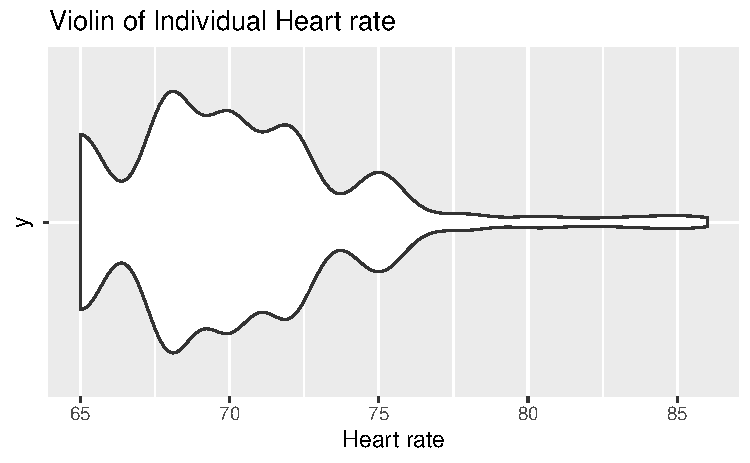
\includegraphics[width=0.7\linewidth]{SleepHelath_files/figure-latex/unnamed-chunk-40-1} \end{center}

\hypertarget{box-plot}{%
\subsection{Box plot}\label{box-plot}}

\begin{Shaded}
\begin{Highlighting}[]
\NormalTok{Sleep\_health\_and\_lifestyle\_dataset\_renamed }\SpecialCharTok{\%\textgreater{}\%}
  \FunctionTok{ggplot}\NormalTok{() }\SpecialCharTok{+}
    \FunctionTok{geom\_boxplot}\NormalTok{(}\AttributeTok{mapping =} \FunctionTok{aes}\NormalTok{(}\AttributeTok{x =}\NormalTok{ HRate)) }\SpecialCharTok{+}
    \FunctionTok{labs}\NormalTok{(}\AttributeTok{title =} \StringTok{"Boxplot of Individual Heart Rate"}\NormalTok{, }\AttributeTok{x =} \StringTok{"Heart rate"}\NormalTok{)}
\end{Highlighting}
\end{Shaded}

\begin{center}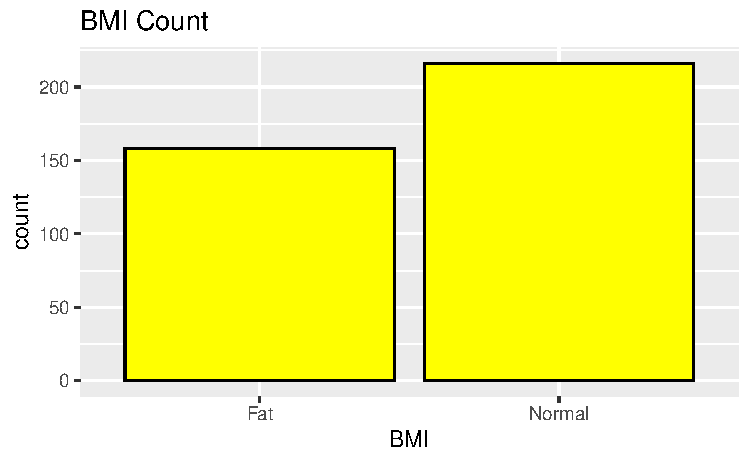
\includegraphics[width=0.7\linewidth]{SleepHelath_files/figure-latex/unnamed-chunk-41-1} \end{center}

\hypertarget{violin-plot}{%
\subsection{Violin plot}\label{violin-plot}}

\begin{Shaded}
\begin{Highlighting}[]
\NormalTok{Sleep\_health\_and\_lifestyle\_dataset\_renamed }\SpecialCharTok{\%\textgreater{}\%}
  \FunctionTok{ggplot}\NormalTok{() }\SpecialCharTok{+}
    \FunctionTok{geom\_violin}\NormalTok{(}\AttributeTok{mapping =} \FunctionTok{aes}\NormalTok{(}\AttributeTok{x =}\NormalTok{ HRate, }\AttributeTok{y =}\StringTok{""}\NormalTok{)) }\SpecialCharTok{+}
    \FunctionTok{labs}\NormalTok{(}\AttributeTok{title =} \StringTok{"Violin of Individual Heart rate"}\NormalTok{, }\AttributeTok{x =} \StringTok{"Heart rate"}\NormalTok{, }\AttributeTok{y =} \StringTok{"y"}\NormalTok{)}
\end{Highlighting}
\end{Shaded}

\begin{center}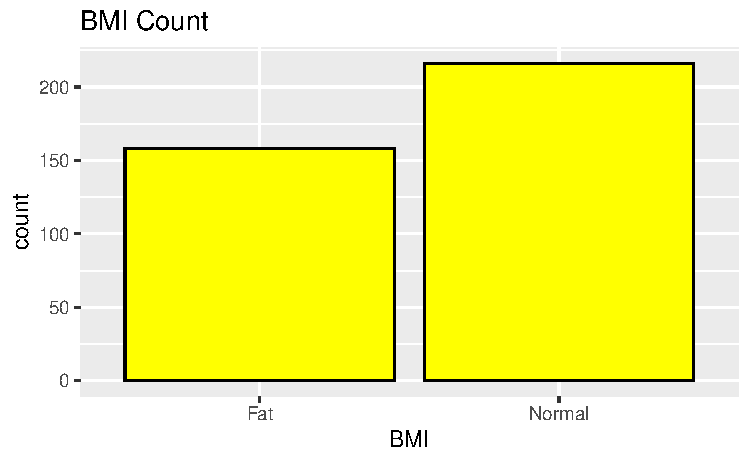
\includegraphics[width=0.7\linewidth]{SleepHelath_files/figure-latex/unnamed-chunk-42-1} \end{center}

\hypertarget{bar-graph}{%
\subsection{Bar Graph}\label{bar-graph}}

\begin{Shaded}
\begin{Highlighting}[]
\NormalTok{Sleep\_health\_and\_lifestyle\_dataset\_renamed }\SpecialCharTok{\%\textgreater{}\%}
  \FunctionTok{ggplot}\NormalTok{() }\SpecialCharTok{+}
    \FunctionTok{geom\_bar}\NormalTok{(}\AttributeTok{mapping =} \FunctionTok{aes}\NormalTok{(}\AttributeTok{x =}\NormalTok{ BMI), }\AttributeTok{color =} \StringTok{"black"}\NormalTok{, }\AttributeTok{fill =} \StringTok{"yellow"}\NormalTok{) }\SpecialCharTok{+}
    \FunctionTok{labs}\NormalTok{(}\AttributeTok{title =} \StringTok{"BMI Count"}\NormalTok{, }\AttributeTok{x =} \StringTok{"BMI"}\NormalTok{)}
\end{Highlighting}
\end{Shaded}

\begin{center}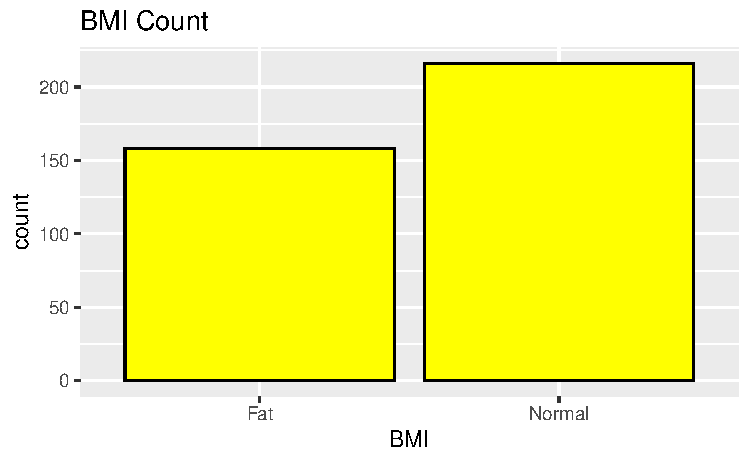
\includegraphics[width=0.7\linewidth]{SleepHelath_files/figure-latex/unnamed-chunk-43-1} \end{center}

\hypertarget{box-plot-1}{%
\subsection{Box plot}\label{box-plot-1}}

\begin{Shaded}
\begin{Highlighting}[]
\NormalTok{Sleep\_health\_and\_lifestyle\_dataset\_renamed }\SpecialCharTok{\%\textgreater{}\%}
  \FunctionTok{ggplot}\NormalTok{() }\SpecialCharTok{+}
    \FunctionTok{geom\_boxplot}\NormalTok{(}\AttributeTok{mapping =} \FunctionTok{aes}\NormalTok{(}\AttributeTok{x =}\NormalTok{ BMI, }\AttributeTok{y =}\NormalTok{ Duration)) }\SpecialCharTok{+}
    \FunctionTok{labs}\NormalTok{(}\AttributeTok{title =} \StringTok{"Relationship between BMI and Duration"}\NormalTok{, }\AttributeTok{x =} \StringTok{"BMI"}\NormalTok{)}
\end{Highlighting}
\end{Shaded}

\begin{center}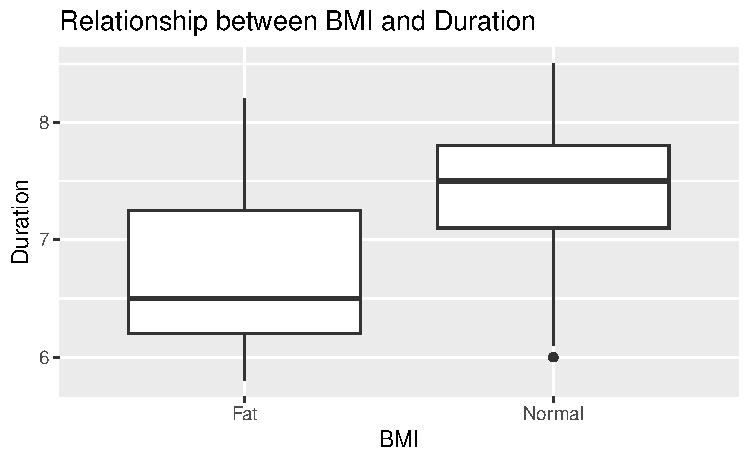
\includegraphics[width=0.7\linewidth]{SleepHelath_files/figure-latex/unnamed-chunk-44-1} \end{center}

\hypertarget{violin-plot-1}{%
\subsection{Violin plot}\label{violin-plot-1}}

\begin{Shaded}
\begin{Highlighting}[]
\NormalTok{Sleep\_health\_and\_lifestyle\_dataset\_renamed }\SpecialCharTok{\%\textgreater{}\%}
  \FunctionTok{ggplot}\NormalTok{() }\SpecialCharTok{+}
    \FunctionTok{geom\_violin}\NormalTok{(}\AttributeTok{mapping =} \FunctionTok{aes}\NormalTok{(}\AttributeTok{x =}\NormalTok{ BMI, }\AttributeTok{y =}\NormalTok{ Duration)) }\SpecialCharTok{+}
    \FunctionTok{labs}\NormalTok{(}\AttributeTok{title =} \StringTok{"Relationship between BMI and Duration"}\NormalTok{, }\AttributeTok{x =} \StringTok{"bmi"}\NormalTok{, }\AttributeTok{y =} \StringTok{"Duration"}\NormalTok{)}
\end{Highlighting}
\end{Shaded}

\begin{center}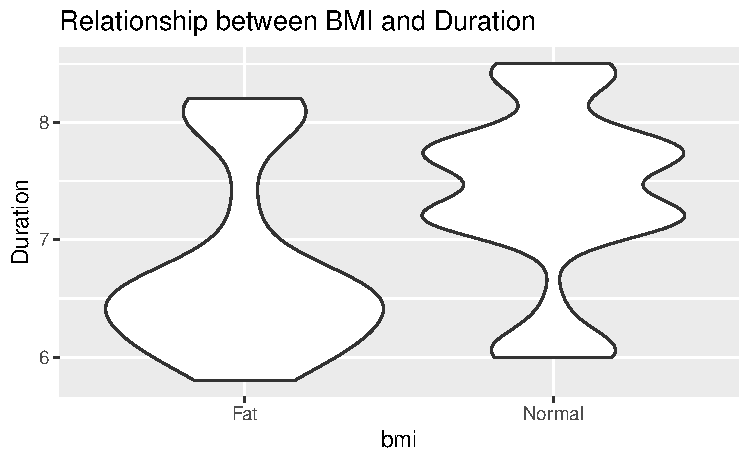
\includegraphics[width=0.7\linewidth]{SleepHelath_files/figure-latex/unnamed-chunk-45-1} \end{center}

\#Scatter plot\_Duration and Heart Rate

\begin{Shaded}
\begin{Highlighting}[]
\NormalTok{Sleep\_health\_and\_lifestyle\_dataset\_renamed    }\SpecialCharTok{\%\textgreater{}\%} 
\FunctionTok{ggplot}\NormalTok{()    }\SpecialCharTok{+}
\FunctionTok{geom\_point}\NormalTok{(}\AttributeTok{mapping =} \FunctionTok{aes}\NormalTok{(}\AttributeTok{x =}\NormalTok{ BMI, }\AttributeTok{y =}\NormalTok{ Duration))    }\SpecialCharTok{+} 
\FunctionTok{labs}\NormalTok{(}
\AttributeTok{title =} \StringTok{"Scatter plot of Duration and Heart Rate"}\NormalTok{, }
\AttributeTok{x =} \StringTok{"BMI"}\NormalTok{,}
\AttributeTok{y =} \StringTok{"Duration"} 
\NormalTok{)}
\end{Highlighting}
\end{Shaded}

\begin{center}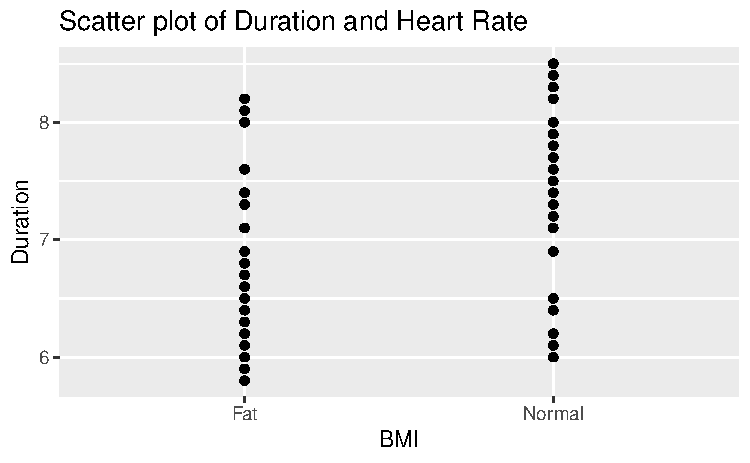
\includegraphics[width=0.7\linewidth]{SleepHelath_files/figure-latex/unnamed-chunk-46-1} \end{center}

\hypertarget{part-5-_-modeling}{%
\subsubsection{PART 5 \_ Modeling}\label{part-5-_-modeling}}

\begin{Shaded}
\begin{Highlighting}[]
\NormalTok{Sleep\_health\_and\_lifestyle\_dataset\_renamed}\SpecialCharTok{\%\textgreater{}\%}
  \FunctionTok{ggplot}\NormalTok{()}\SpecialCharTok{+}
  \FunctionTok{geom\_point}\NormalTok{( }\AttributeTok{mapping =} \FunctionTok{aes}\NormalTok{( }\AttributeTok{x  =}\NormalTok{ Physical , }\AttributeTok{y =}\NormalTok{ Duration)) }\SpecialCharTok{+}
  \FunctionTok{labs}\NormalTok{(}\AttributeTok{title =} \StringTok{"Relationships between Physical activies and Duration"}\NormalTok{,}
       \AttributeTok{x =} \StringTok{"Physical Activities"}\NormalTok{ , }\AttributeTok{y =} \StringTok{"Duration"}\NormalTok{)}
\end{Highlighting}
\end{Shaded}

\begin{center}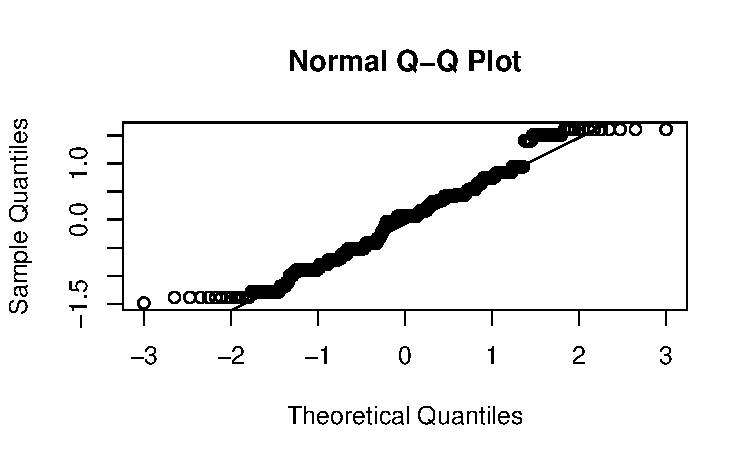
\includegraphics[width=0.7\linewidth]{SleepHelath_files/figure-latex/unnamed-chunk-47-1} \end{center}

\begin{Shaded}
\begin{Highlighting}[]
\NormalTok{data }\OtherTok{\textless{}{-}}\NormalTok{ Sleep\_health\_and\_lifestyle\_dataset\_renamed}

\NormalTok{model }\OtherTok{\textless{}{-}} \FunctionTok{lm}\NormalTok{(Duration }\SpecialCharTok{\textasciitilde{}}\NormalTok{ Physical, }\AttributeTok{data =}\NormalTok{ Sleep\_health\_and\_lifestyle\_dataset\_renamed)}


\FunctionTok{summary}\NormalTok{(model)}
\end{Highlighting}
\end{Shaded}

\begin{verbatim}
## 
## Call:
## lm(formula = Duration ~ Physical, data = Sleep_health_and_lifestyle_dataset_renamed)
## 
## Residuals:
##      Min       1Q   Median       3Q      Max 
## -1.48215 -0.59686  0.06119  0.43952  1.60453 
## 
## Coefficients:
##             Estimate Std. Error t value Pr(>|t|)    
## (Intercept) 6.652128   0.121379  54.805  < 2e-16 ***
## Physical    0.008111   0.001935   4.191 3.47e-05 ***
## ---
## Signif. codes:  0 '***' 0.001 '**' 0.01 '*' 0.05 '.' 0.1 ' ' 1
## 
## Residual standard error: 0.7786 on 372 degrees of freedom
## Multiple R-squared:  0.0451, Adjusted R-squared:  0.04253 
## F-statistic: 17.57 on 1 and 372 DF,  p-value: 3.467e-05
\end{verbatim}

\begin{Shaded}
\begin{Highlighting}[]
\NormalTok{residuals }\OtherTok{\textless{}{-}} \FunctionTok{residuals}\NormalTok{(model)}

\FunctionTok{qqnorm}\NormalTok{(residuals)}
\FunctionTok{qqline}\NormalTok{(residuals)}
\end{Highlighting}
\end{Shaded}

\begin{center}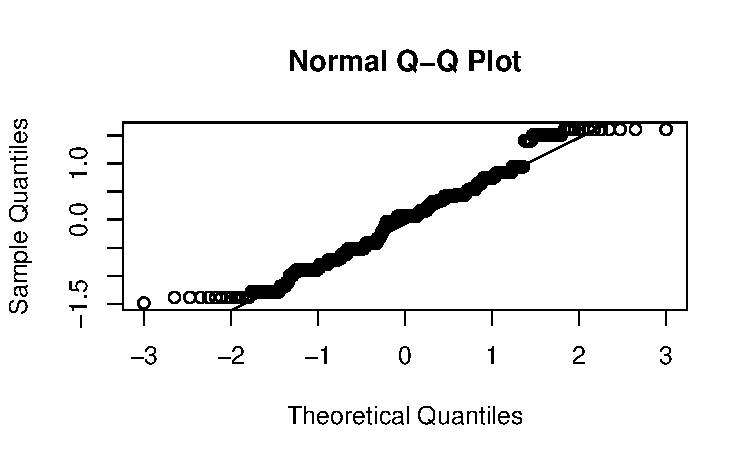
\includegraphics[width=0.7\linewidth]{SleepHelath_files/figure-latex/unnamed-chunk-49-1} \end{center}

\begin{Shaded}
\begin{Highlighting}[]
\FunctionTok{labs}\NormalTok{( }\AttributeTok{title  =} \StringTok{"QQplot"}\NormalTok{ , }\AttributeTok{x =} \StringTok{"Theoretical"}\NormalTok{ , }\AttributeTok{y =} \StringTok{"Quantaties"}\NormalTok{)}
\end{Highlighting}
\end{Shaded}

\begin{verbatim}
## $x
## [1] "Theoretical"
## 
## $y
## [1] "Quantaties"
## 
## $title
## [1] "QQplot"
## 
## attr(,"class")
## [1] "labels"
\end{verbatim}

\begin{Shaded}
\begin{Highlighting}[]
\NormalTok{Renamed\_other\_model }\OtherTok{\textless{}{-}} \FunctionTok{lm}\NormalTok{(Duration }\SpecialCharTok{\textasciitilde{}}\NormalTok{ Physical, }\AttributeTok{data =}\NormalTok{ Sleep\_health\_and\_lifestyle\_dataset\_renamed)}
\end{Highlighting}
\end{Shaded}

\begin{Shaded}
\begin{Highlighting}[]
\NormalTok{Renamed\_other\_model}\SpecialCharTok{$}\NormalTok{coefficients}
\end{Highlighting}
\end{Shaded}

\begin{verbatim}
## (Intercept)    Physical 
## 6.652127945 0.008111349
\end{verbatim}

\begin{Shaded}
\begin{Highlighting}[]
\NormalTok{Renamed\_other\_model}\SpecialCharTok{\%\textgreater{}\%}
  \FunctionTok{tidy}\NormalTok{()}
\end{Highlighting}
\end{Shaded}

\begin{longtable}[]{@{}lrrrr@{}}
\toprule\noalign{}
term & estimate & std.error & statistic & p.value \\
\midrule\noalign{}
\endhead
\bottomrule\noalign{}
\endlastfoot
(Intercept) & 6.6521279 & 0.1213792 & 54.804523 & 0.00e+00 \\
Physical & 0.0081113 & 0.0019352 & 4.191459 & 3.47e-05 \\
\end{longtable}

\begin{Shaded}
\begin{Highlighting}[]
\NormalTok{Renamed\_other\_model}\SpecialCharTok{\%\textgreater{}\%}
  \FunctionTok{glance}\NormalTok{()}\SpecialCharTok{\%\textgreater{}\%}
  \FunctionTok{select}\NormalTok{(r.squared)}
\end{Highlighting}
\end{Shaded}

\begin{longtable}[]{@{}r@{}}
\toprule\noalign{}
r.squared \\
\midrule\noalign{}
\endhead
\bottomrule\noalign{}
\endlastfoot
0.0450969 \\
\end{longtable}

\begin{Shaded}
\begin{Highlighting}[]
\NormalTok{Sleep\_health\_and\_lifestyle\_dataset\_renamed}\SpecialCharTok{\%\textgreater{}\%}
  \FunctionTok{ggplot}\NormalTok{()}\SpecialCharTok{+}
  \FunctionTok{geom\_point}\NormalTok{(}\AttributeTok{mapping =} \FunctionTok{aes}\NormalTok{( }\AttributeTok{x  =}\NormalTok{ Physical , }\AttributeTok{y =}\NormalTok{ Duration) )}\SpecialCharTok{+}
  \FunctionTok{geom\_abline}\NormalTok{(}\AttributeTok{slope =}\NormalTok{ Renamed\_other\_model}\SpecialCharTok{$}\NormalTok{coefficients[}\DecValTok{2}\NormalTok{]   ,}
              \AttributeTok{intercept =}\NormalTok{ Renamed\_other\_model}\SpecialCharTok{$}\NormalTok{coefficients[}\DecValTok{1}\NormalTok{]  )}\SpecialCharTok{+}
  \FunctionTok{labs}\NormalTok{( }\AttributeTok{title =} \StringTok{"Relationships between Physical and Duration"}\NormalTok{,}
        \AttributeTok{x =} \StringTok{" Physical "}\NormalTok{,}
        \AttributeTok{y =} \StringTok{" Duration"}\NormalTok{ )}
\end{Highlighting}
\end{Shaded}

\begin{center}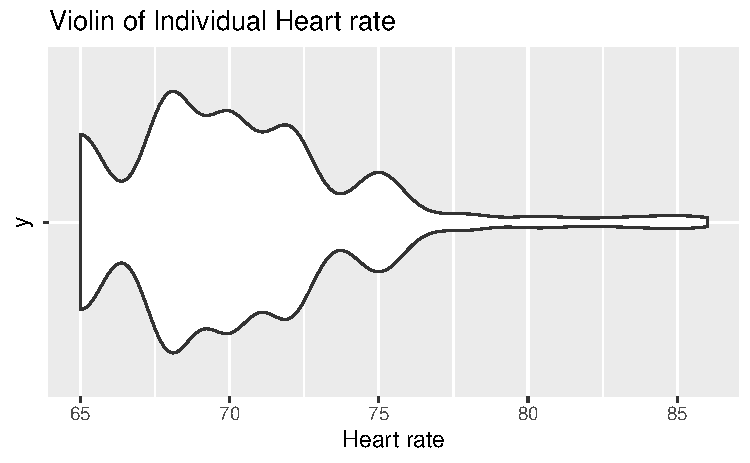
\includegraphics[width=0.7\linewidth]{SleepHelath_files/figure-latex/unnamed-chunk-54-1} \end{center}

\#Advanced Modeling

\begin{Shaded}
\begin{Highlighting}[]
\NormalTok{continuous\_model }\OtherTok{\textless{}{-}} \FunctionTok{lm}\NormalTok{(Duration }\SpecialCharTok{\textasciitilde{}}\NormalTok{ Gender }\SpecialCharTok{+}\NormalTok{ Age }\SpecialCharTok{+}\NormalTok{ Occupation }\SpecialCharTok{+}\NormalTok{ DSteps }\SpecialCharTok{+}\NormalTok{ BMI }\SpecialCharTok{+}\NormalTok{ Physical, }\AttributeTok{data =}\NormalTok{ Sleep\_health\_and\_lifestyle\_dataset\_renamed)}
\NormalTok{coefficients }\OtherTok{\textless{}{-}} \FunctionTok{tidy}\NormalTok{ (continuous\_model)}
\NormalTok{coefficients}
\end{Highlighting}
\end{Shaded}

\begin{longtable}[]{@{}
  >{\raggedright\arraybackslash}p{(\columnwidth - 8\tabcolsep) * \real{0.4189}}
  >{\raggedleft\arraybackslash}p{(\columnwidth - 8\tabcolsep) * \real{0.1486}}
  >{\raggedleft\arraybackslash}p{(\columnwidth - 8\tabcolsep) * \real{0.1351}}
  >{\raggedleft\arraybackslash}p{(\columnwidth - 8\tabcolsep) * \real{0.1622}}
  >{\raggedleft\arraybackslash}p{(\columnwidth - 8\tabcolsep) * \real{0.1351}}@{}}
\toprule\noalign{}
\begin{minipage}[b]{\linewidth}\raggedright
term
\end{minipage} & \begin{minipage}[b]{\linewidth}\raggedleft
estimate
\end{minipage} & \begin{minipage}[b]{\linewidth}\raggedleft
std.error
\end{minipage} & \begin{minipage}[b]{\linewidth}\raggedleft
statistic
\end{minipage} & \begin{minipage}[b]{\linewidth}\raggedleft
p.value
\end{minipage} \\
\midrule\noalign{}
\endhead
\bottomrule\noalign{}
\endlastfoot
(Intercept) & 3.8296315 & 0.3275001 & 11.6935269 & 0.0000000 \\
GenderMale & -0.1949526 & 0.1287189 & -1.5145603 & 0.1307662 \\
Age & 0.0655149 & 0.0062353 & 10.5071674 & 0.0000000 \\
OccupationDoctor & 0.4245451 & 0.1384180 & 3.0671237 & 0.0023258 \\
OccupationEngineer & 0.3033566 & 0.1400149 & 2.1666029 & 0.0309244 \\
OccupationLawyer & 0.2877110 & 0.1525615 & 1.8858691 & 0.0601220 \\
OccupationManager & 0.1297888 & 0.4617227 & 0.2810969 & 0.7787985 \\
OccupationNurse & -0.2098419 & 0.1178946 & -1.7799108 & 0.0759387 \\
OccupationSales Representative & 0.4350443 & 0.3563943 & 1.2206825 &
0.2230096 \\
OccupationSalesperson & 0.3071433 & 0.1756392 & 1.7487178 & 0.0811969 \\
OccupationScientist & 0.3016381 & 0.2640060 & 1.1425423 & 0.2539922 \\
OccupationSoftware Engineer & 0.7486436 & 0.2586419 & 2.8945175 &
0.0040302 \\
OccupationTeacher & 0.3402722 & 0.1224097 & 2.7797809 & 0.0057268 \\
DSteps & -0.0002563 & 0.0000246 & -10.4369782 & 0.0000000 \\
BMINormal & 1.1644995 & 0.1087480 & 10.7082352 & 0.0000000 \\
Physical & 0.0254908 & 0.0020941 & 12.1729446 & 0.0000000 \\
\end{longtable}

\begin{Shaded}
\begin{Highlighting}[]
\NormalTok{r\_squared }\OtherTok{\textless{}{-}} \FunctionTok{glance}\NormalTok{(continuous\_model)}\SpecialCharTok{$}\NormalTok{r.squared}
\end{Highlighting}
\end{Shaded}

\begin{Shaded}
\begin{Highlighting}[]
\NormalTok{Sleep\_health\_and\_lifestyle\_dataset\_df }\OtherTok{\textless{}{-}}\NormalTok{ Sleep\_health\_and\_lifestyle\_dataset\_renamed }\SpecialCharTok{\%\textgreater{}\%}
  \FunctionTok{add\_predictions}\NormalTok{(continuous\_model) }\SpecialCharTok{\%\textgreater{}\%}
  \FunctionTok{add\_residuals}\NormalTok{(continuous\_model)}
\end{Highlighting}
\end{Shaded}

\#Histogram of residual in Sleep\_health\_and\_lifestyle\_dataset\_df

\begin{Shaded}
\begin{Highlighting}[]
\NormalTok{Sleep\_health\_and\_lifestyle\_dataset\_df }\SpecialCharTok{\%\textgreater{}\%}
  \FunctionTok{ggplot}\NormalTok{() }\SpecialCharTok{+}
  \FunctionTok{geom\_histogram}\NormalTok{(}\AttributeTok{mapping =} \FunctionTok{aes}\NormalTok{(}\AttributeTok{x =}\NormalTok{ resid), }\AttributeTok{color =} \StringTok{"blue"}\NormalTok{, }\AttributeTok{fill =} \StringTok{"pink"}\NormalTok{, }\AttributeTok{bins =} \DecValTok{10}\NormalTok{) }\SpecialCharTok{+}
  \FunctionTok{labs}\NormalTok{(}\AttributeTok{x =} \StringTok{"residual"}\NormalTok{, }\AttributeTok{y =}\StringTok{"Duration"}\NormalTok{,}
\AttributeTok{title =} \StringTok{"Histogram of residual in Sleep\_health\_and\_lifestyle\_dataset\_df"}\NormalTok{)}
\end{Highlighting}
\end{Shaded}

\begin{center}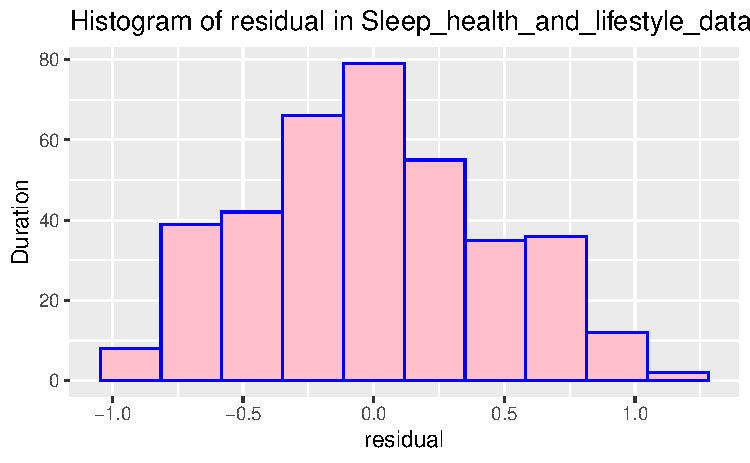
\includegraphics[width=0.7\linewidth]{SleepHelath_files/figure-latex/unnamed-chunk-58-1} \end{center}

\#Observed vs.~Predicted Plot

\begin{Shaded}
\begin{Highlighting}[]
\NormalTok{Sleep\_health\_and\_lifestyle\_dataset\_df }\SpecialCharTok{\%\textgreater{}\%}
  \FunctionTok{ggplot}\NormalTok{() }\SpecialCharTok{+}
  \FunctionTok{geom\_point}\NormalTok{(}\AttributeTok{mapping =} \FunctionTok{aes}\NormalTok{(}\AttributeTok{x =}\NormalTok{ pred, }\AttributeTok{y =}\NormalTok{ Duration)) }\SpecialCharTok{+}
  \FunctionTok{geom\_abline}\NormalTok{(}\AttributeTok{slope =} \DecValTok{1}\NormalTok{, }\AttributeTok{intercept =} \DecValTok{0}\NormalTok{) }\SpecialCharTok{+}
  \FunctionTok{labs}\NormalTok{(}\AttributeTok{title =} \StringTok{"Observed vs. Predicted Plot"}\NormalTok{, }\AttributeTok{x =} \StringTok{"Predicted Duration"}\NormalTok{, }\AttributeTok{y =} \StringTok{"Observed Duration"}\NormalTok{)}
\end{Highlighting}
\end{Shaded}

\begin{center}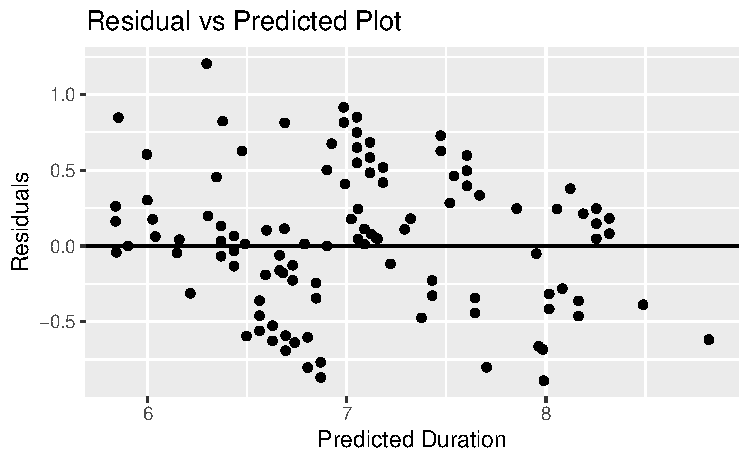
\includegraphics[width=0.7\linewidth]{SleepHelath_files/figure-latex/unnamed-chunk-59-1} \end{center}

\#Residual vs Predicted Plot

\begin{Shaded}
\begin{Highlighting}[]
\NormalTok{Sleep\_health\_and\_lifestyle\_dataset\_df }\SpecialCharTok{\%\textgreater{}\%}
  \FunctionTok{ggplot}\NormalTok{() }\SpecialCharTok{+}
  \FunctionTok{geom\_point}\NormalTok{(}\AttributeTok{mapping =} \FunctionTok{aes}\NormalTok{(}\AttributeTok{x =}\NormalTok{ pred, }\AttributeTok{y =}\NormalTok{ resid)) }\SpecialCharTok{+}
  \FunctionTok{geom\_hline}\NormalTok{(}\AttributeTok{yintercept =} \DecValTok{0}\NormalTok{) }\SpecialCharTok{+}
  \FunctionTok{labs}\NormalTok{( }\AttributeTok{title=} \StringTok{"Residual vs Predicted Plot"}\NormalTok{,}
        \AttributeTok{x =} \StringTok{"Predicted Duration"}\NormalTok{,}
        \AttributeTok{y =} \StringTok{"Residuals"}\NormalTok{)}
\end{Highlighting}
\end{Shaded}

\begin{center}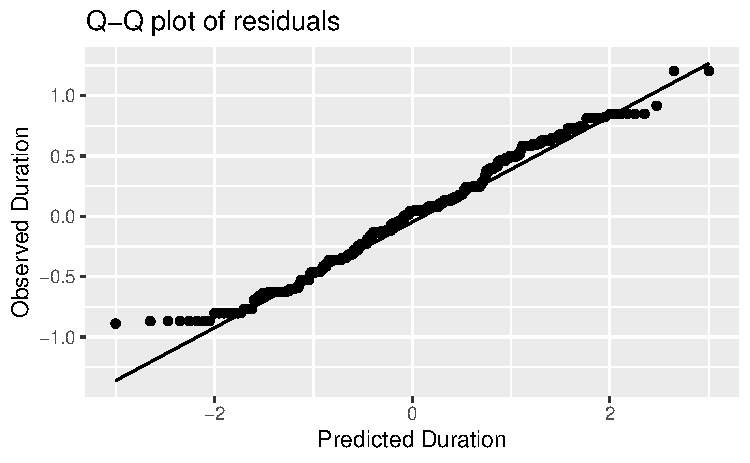
\includegraphics[width=0.7\linewidth]{SleepHelath_files/figure-latex/unnamed-chunk-60-1} \end{center}

\#Q-Q Plot (Obeserved vs Predicted Plot)

\begin{Shaded}
\begin{Highlighting}[]
\NormalTok{Sleep\_health\_and\_lifestyle\_dataset\_df }\SpecialCharTok{\%\textgreater{}\%}
  \FunctionTok{ggplot}\NormalTok{() }\SpecialCharTok{+}
  \FunctionTok{geom\_qq}\NormalTok{(}\FunctionTok{aes}\NormalTok{(}\AttributeTok{sample =}\NormalTok{ resid)) }\SpecialCharTok{+}
  \FunctionTok{geom\_qq\_line}\NormalTok{(}\FunctionTok{aes}\NormalTok{(}\AttributeTok{sample =}\NormalTok{ resid))}\SpecialCharTok{+}
  \FunctionTok{labs}\NormalTok{(}\AttributeTok{title =} \StringTok{"Q{-}Q plot of residuals"}\NormalTok{, }\AttributeTok{x=} \StringTok{"Predicted Duration"}\NormalTok{, }\AttributeTok{y=} \StringTok{"Observed Duration"}\NormalTok{)}
\end{Highlighting}
\end{Shaded}

\begin{center}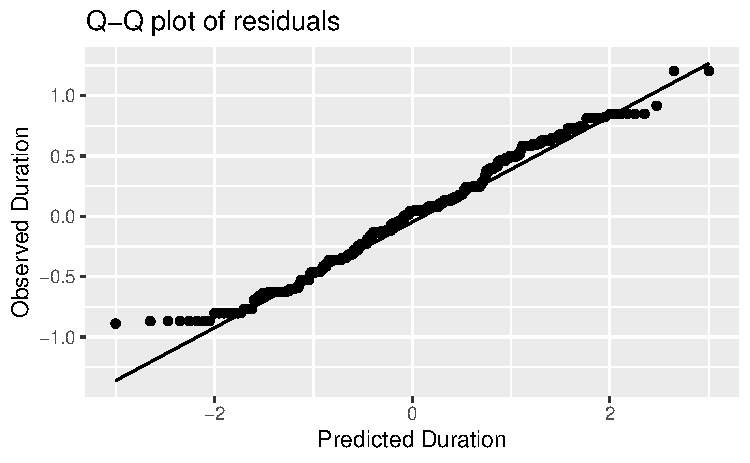
\includegraphics[width=0.7\linewidth]{SleepHelath_files/figure-latex/unnamed-chunk-61-1} \end{center}

\#Box Plot

\begin{Shaded}
\begin{Highlighting}[]
\NormalTok{Sleep\_health\_and\_lifestyle\_dataset\_df }\SpecialCharTok{\%\textgreater{}\%}
  \FunctionTok{pivot\_longer}\NormalTok{(}
    \AttributeTok{cols =}\NormalTok{ Gender}\SpecialCharTok{:}\NormalTok{Occupation }\SpecialCharTok{|}\NormalTok{ Physical }\SpecialCharTok{|}\NormalTok{ BMI }\SpecialCharTok{|}\NormalTok{ DSteps,}
    \AttributeTok{names\_to =} \StringTok{"column"}\NormalTok{,}
    \AttributeTok{values\_to =} \StringTok{"value"}\NormalTok{,}
    \AttributeTok{values\_transform =} \FunctionTok{list}\NormalTok{(}\AttributeTok{value =} \StringTok{\textquotesingle{}factor\textquotesingle{}}\NormalTok{)}
\NormalTok{) }\SpecialCharTok{\%\textgreater{}\%}
\FunctionTok{ggplot}\NormalTok{() }\SpecialCharTok{+}
  \FunctionTok{geom\_boxplot}\NormalTok{(}\FunctionTok{aes}\NormalTok{(}\AttributeTok{x =} \FunctionTok{reorder}\NormalTok{(value, Duration, }\AttributeTok{FUN =}\NormalTok{ median), }\AttributeTok{y =}\NormalTok{ Duration)) }\SpecialCharTok{+}
  \FunctionTok{facet\_wrap}\NormalTok{(}\SpecialCharTok{\textasciitilde{}}\NormalTok{column, }\AttributeTok{scales =} \StringTok{"free\_x"}\NormalTok{) }\SpecialCharTok{+}
  \FunctionTok{labs}\NormalTok{(}\AttributeTok{x =} \StringTok{"x variable"}\NormalTok{, }\AttributeTok{y =} \StringTok{"Duration"}\NormalTok{, }\AttributeTok{title =} \StringTok{"Box Plot of x variables"}\NormalTok{) }\SpecialCharTok{+}
  \FunctionTok{theme}\NormalTok{(}\AttributeTok{axis.text.x =} \FunctionTok{element\_text}\NormalTok{(}\AttributeTok{angle =} \DecValTok{45}\NormalTok{))}
\end{Highlighting}
\end{Shaded}

\begin{center}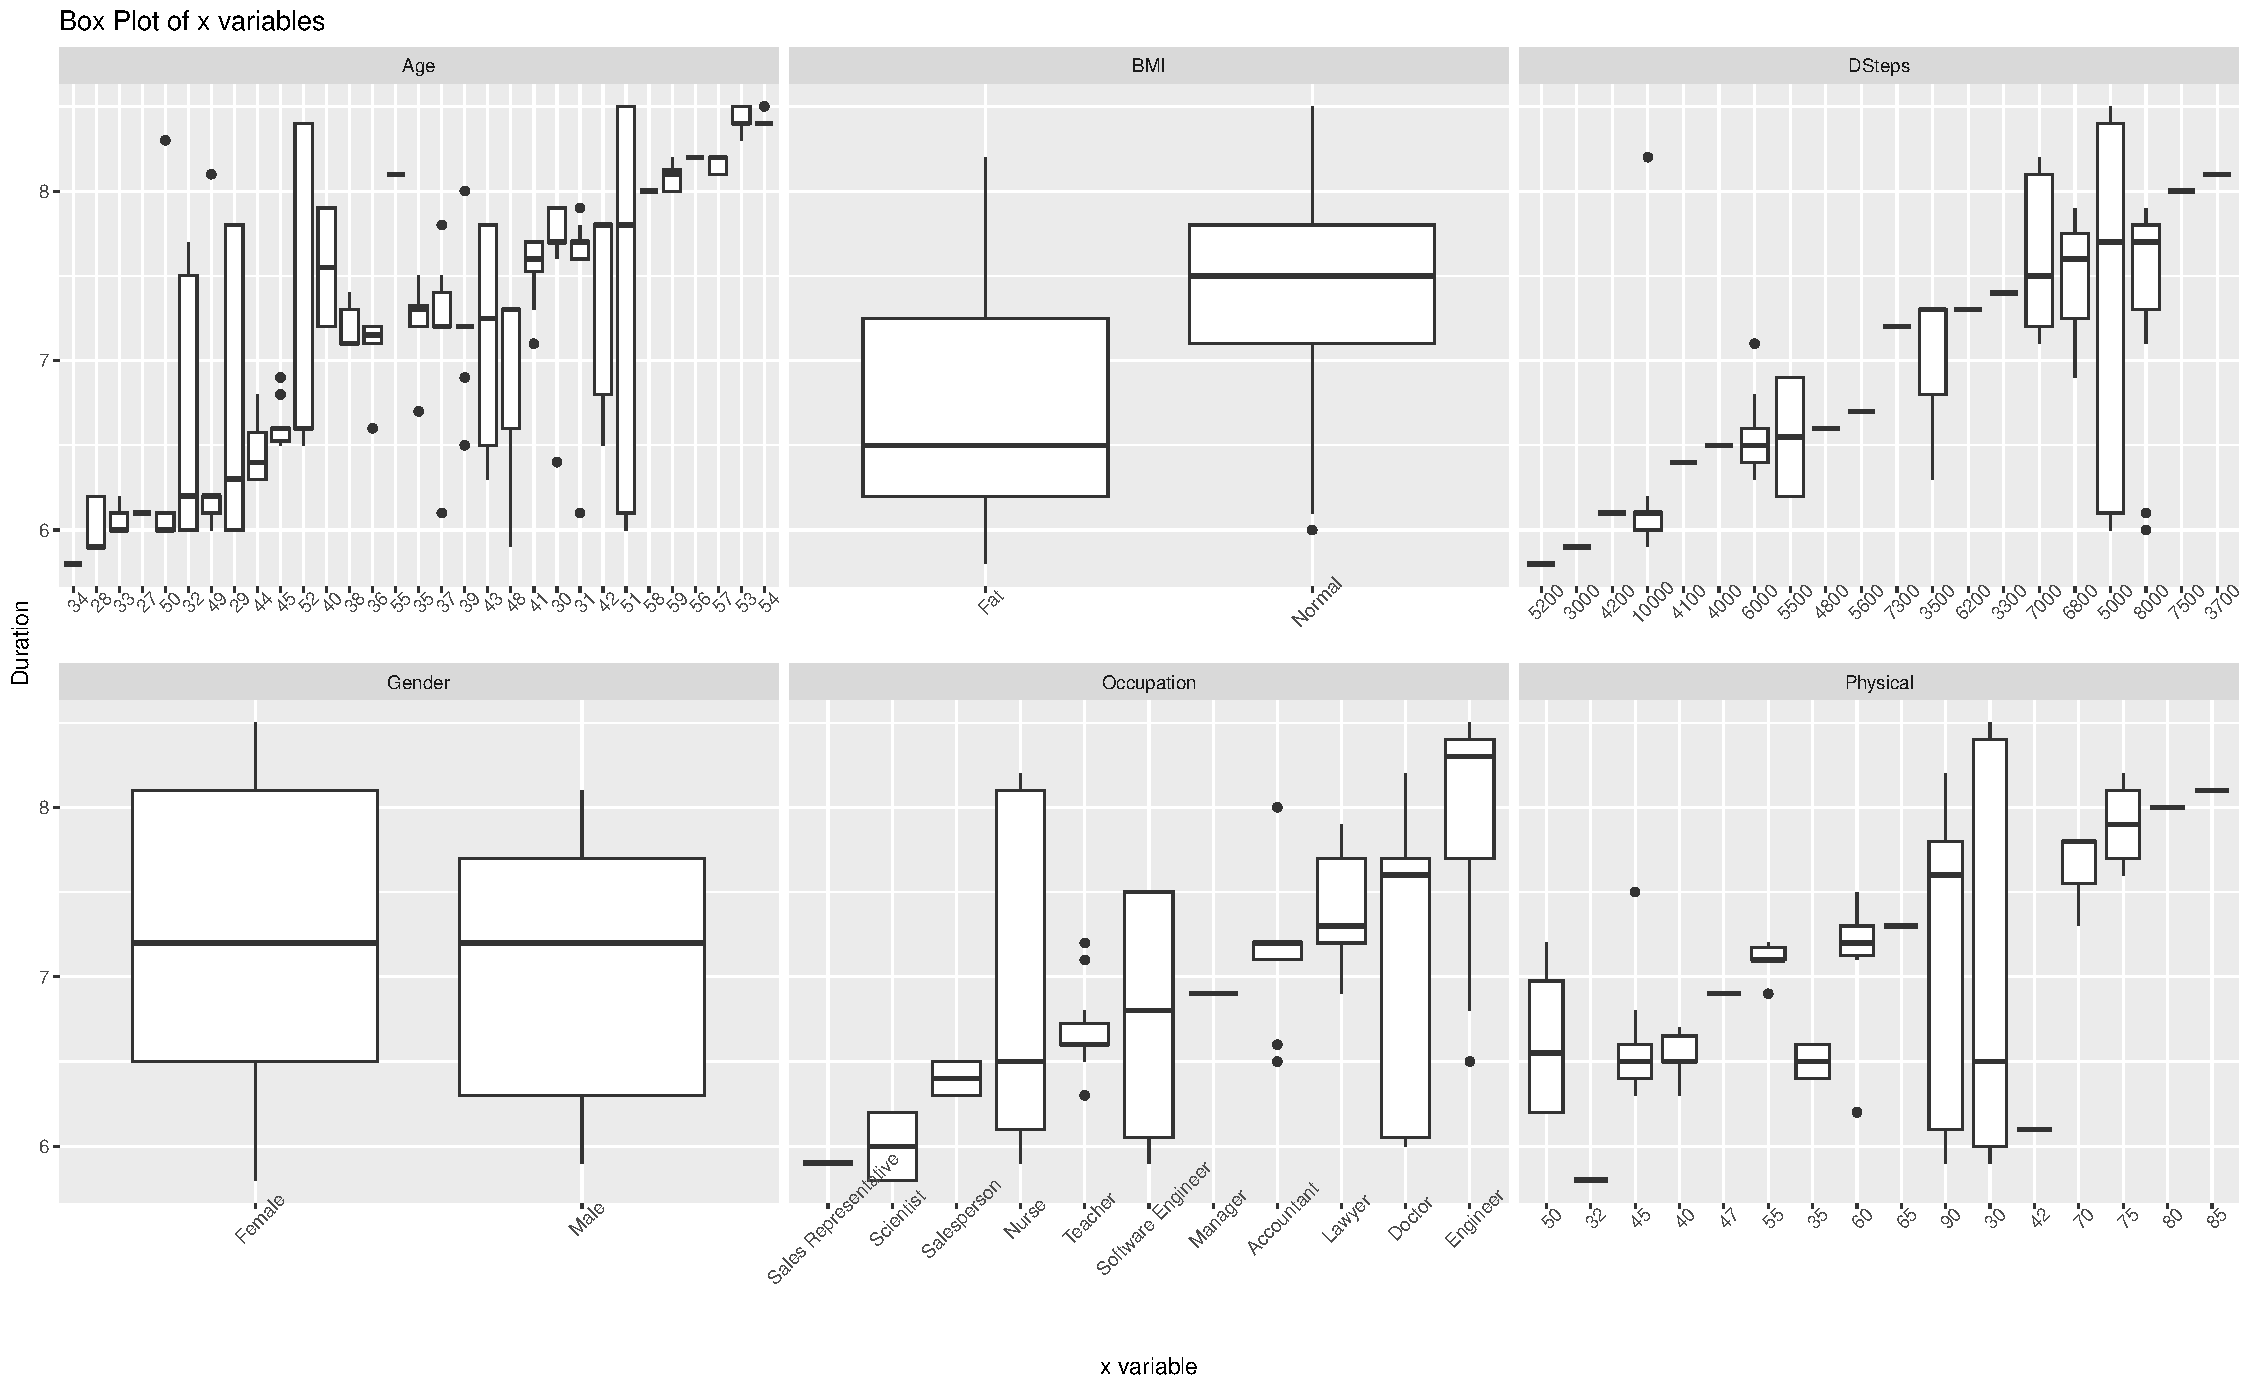
\includegraphics[width=0.7\linewidth]{SleepHelath_files/figure-latex/unnamed-chunk-62-1} \end{center}

\end{document}
